\documentclass[12pt, a4paper]{report}

\usepackage{geometry}
\geometry{left=1.5in, right=1in, top=1in, bottom=1in}

\usepackage{setspace}
\renewcommand{\baselinestretch}{1.32}

% ==================== 2. FONTS & LANGUAGE ====================
\usepackage{fontspec}
\usepackage{polyglossia}

\setdefaultlanguage{english}
\setotherlanguage{sanskrit}

\newfontfamily\devanagarifont{NotoSerifDevanagari-Regular}[
    Path = /usr/share/fonts/google-noto/,
    Extension = .ttf,
    Scale = 1.0,
    Script = Devanagari,
    BoldFont = NotoSerifDevanagari-Bold,
]
\newcommand{\dev}[1]{{\devanagarifont #1}}

% ==================== 3. ESSENTIAL PACKAGES ====================
\usepackage{amsmath}
\usepackage{amssymb}
\usepackage{graphicx}
\usepackage{xcolor}
\usepackage{float}
\usepackage{booktabs}
\usepackage{longtable}
\usepackage{array}
\usepackage{caption}
\usepackage{subcaption}
\usepackage{enumitem}
\usepackage{fancyhdr}
\usepackage{titlesec}
\usepackage[square,numbers,comma,sort&compress]{natbib}
\usepackage[hidelinks]{hyperref}
\usepackage[titles]{tocloft}

% ---------- LIST OF FIGURES / TABLES formatting ----------
% Smaller font for entries
\renewcommand{\cftfigfont}{\footnotesize}
\renewcommand{\cftfigpagefont}{\footnotesize}
\renewcommand{\cfttabfont}{\footnotesize}
\renewcommand{\cfttabpagefont}{\footnotesize}
% Extra vertical space between entries
\setlength{\cftbeforefigskip}{6pt}
\setlength{\cftbeforetabskip}{6pt}

% ---------- HEADER & FOOTER (fancyhdr) ----------
\pagestyle{fancy}
\setlength{\headheight}{14.5pt}
\lhead{\leftmark}
\rhead{\thepage}
\cfoot{}
\renewcommand{\headrulewidth}{0.4pt} % Adds the horizontal line at the top

% ==================== DOCUMENT START ====================
\begin{document}

% ---------- FRONT MATTER ----------
\pagenumbering{roman}
\begin{titlepage}
	\vspace{50pt}
	\begin{center}
		\makebox[\textwidth]{%
			\parbox{1.15\textwidth}{\centering\Large\bf BYT5-SANSKRIT WITH BALANCED REGULARIZATION FOR SANSKRIT NAMED ENTITY RECOGNITION}}
	\end{center}

	\begin{center}
		{
			A thesis submitted in partial fulfillment of \\the requirements for the degree of \\Master of Technology 
			}\\
		in\\
		Modelling \& Simulation\\
		\vspace{10pt}
		{BY}\\
		{\large\bf Yogesh}\\
		(Roll No. 24-14-15)\\
		\vspace{30pt}
		{UNDER THE SUPERVISION OF}\\
		{\large\bf Dr. Somanchi V. S. S. N. V. G. Krishna Murthy\\}(Supervisor \& Professor-DIAT)
	\end{center}
	\vspace*{\fill}
	\begin{center}
		
\includegraphics[scale=0.5]{images/DIATlogo.png}
	\end{center}
	\vspace*{\fill}
	\begin{center}
		{\bf
			Department of Applied Mathematics} \\{\large\bf
            Defence Institute of Advanced Technology\\(Deemed to be University)\\Girinagar, Pune - 411025\\}
	\end{center}
	\begin{center}
		{\large \bf MAY 2026}
	\end{center}
\end{titlepage}
\clearpage
\thispagestyle{plain}
\addcontentsline{toc}{chapter}{Certificate}
\begin{center}
{\large\bfseries C E R T I F I C A T E}
\end{center}

\vspace{10mm}

\noindent
This is to certify that the Thesis entitled 
\textbf{``BYT5-SANSKRIT WITH BALANCED REGULARIZATION FOR SANSKRIT NAMED ENTITY RECOGNITION''} submitted to Defence Institute of Advanced Technology, Girinagar, for the award of the degree of 
\textbf{Master of Technology}, is the bonafide research work done by 
\textbf{Mr. YOGESH} under my supervision. 
The contents of this thesis have not been submitted elsewhere for the award of any degree.

\vspace{25mm}

\begin{minipage}[t]{0.55\textwidth}
    \raggedright \small
    \textbf{Dr. S.V.S.S.N.V.G. Krishna Murthy} \\[0.1cm]
    Supervisor \& Professor, \\[0.1cm]
    Department of Applied Mathematics, \\[0.1cm]
    Defence Institute of Advanced Technology, \\[0.1cm]
   %  (Deemed to be University), \\
    Pune - 411025\\[0.1cm]
\end{minipage}
\hfill 
\begin{minipage}[t]{0.48\textwidth}
    % Left blank as there is no external guide
\end{minipage}

\vspace{15mm}

\begin{center}
\textbf{COUNTERSIGNED BY}
\end{center}

\vspace{25mm}

\begin{center} \textbf{Dr. Odelu Ojjela} \\ 
    Professor \& Head, \\ 
    Department of Applied Mathematics, \\ 
    Defence Institute of Advanced Technology, \\ 
    %(Deemed to be University), \\
    Pune - 411025 
\end{center}
\clearpage
\addcontentsline{toc}{chapter}{Declaration}

\begin{center}
{\bfseries DECLARATION}\\[5ex]
\end{center}

\noindent This is to certify that the work presented in the Thesis entitled
{\bfseries ``BYT5-SANSKRIT WITH BALANCED REGULARIZATION FOR SANSKRIT NAMED ENTITY RECOGNITION''},
is a bonafide work done by me under the supervision of
{\bfseries Dr. S.V.S.S.N.V.G. Krishna Murthy}
and has not been submitted elsewhere for the award of any degree.

\vspace{0.8in}

\noindent
\begin{minipage}[t]{0.45\textwidth}
\textbf{Date:}\rule[-3pt]{1.3in}{0.5pt}\\[1.5ex]
\textbf{Place:}\rule[-3pt]{1.3in}{0.5pt}
\end{minipage}
\hfill
\begin{minipage}[t]{0.60\textwidth}
Name: Yogesh\\
Roll No.: 24-14-15\\
Department of Applied Mathematics\\
Defence Institute of Advanced Technology\\
Pune - 411025
\end{minipage}

\vspace{1.0in}

\begin{center}
{\bfseries COUNTERSIGNED}
\end{center}

\vspace{1.0in}

\noindent
\begin{minipage}[t]{0.55\textwidth}
Dr. S.V.S.S.N.V.G. Krishna Murthy\\[1ex]
Professor\\[1ex]
Department of Applied Mathematics\\[1ex]
Defence Institute of Advanced Technology\\[1ex]
Pune - 411025
\end{minipage}
\hfill
\begin{minipage}[t]{0.48\textwidth}
% Left blank as there is no external guide
\end{minipage}
\addcontentsline{toc}{chapter}{Acknowledgements}
\begin{center}
{\bf A C K N O W L E D G E M E N T S}
\end{center}
\vspace{0.8cm}
I would like to express my sincere gratitude to my supervisors, Dr. S.V.S.S.N.V.G.
Krishna Murthy, for their invaluable guidance, feedback, and
encouragement throughout the initial stages of this research. Their insights and expertise have been instrumental in shaping the direction and methodology of this work, and I am deeply thankful for their support.

I am grateful to the Defence Institute of Advanced Technology, Pune, and the Department of Applied Mathematics for providing the facilities, resources, and academic
environment necessary to undertake this study.

My heartfelt thanks extend to my peers and colleagues for their thoughtful discussions
and assistance, which have helped refine the concepts and methodologies explored in this phase of the research.

I am also profoundly thankful to my family and friends for their unwavering support and
motivation, which have been a source of strength during this ongoing journey.
Lastly, I would like to acknowledge the developers and contributors of open-source platforms and tools, which have been vital for the experimental work conducted thus far.

This report marks an important milestone in my research, and I am grateful to all who
have contributed to its progress.
\addcontentsline{toc}{chapter}{Approval Sheet}
\begin{center}
	{\Large \textbf{APPROVAL SHEET}}
\end{center}

\vspace{0.5em}
\vspace{1cm}
\noindent
%\renewcommand{\arraystretch}{1.5} % Adjusts the overall row height

\begin{tabular}{@{}p{4cm} p{10cm}@{}}
	{Title of the thesis:} & \setstretch{1.32}\textbf{Byt5-Sanskrit With Balanced Regularization For Sanskrit Named Entity Recognition}
\end{tabular}\\[.5em]
\indent Candidate's Name:    \textbf{Yogesh (Reg. No. 24-14-15)} is approved for the degree \indent of \textbf{Master of Technology in Modeling \& Simulation}.

%\end{tabular}

%\vspace{0.8em}
%\noindent
%is approved for the degree of \textbf{Master of Technology in Modeling \& Simulation}.
%

\begin{center}
	\textbf{Examiners:}
\end{center}
\vspace{3.5em}
\vspace{1cm}
\noindent\hfill
\begin{minipage}[t]{9cm}
	\centering
	\rule{9cm}{0.4pt}\\[0.3em]
	\textbf{Supervisor}\\
	%\textbf{(Dr. S.V.S.S.N.V.G. Krishna Murthy)}
\end{minipage}

\vspace{3.5em}
\vspace{1cm}
\noindent\hfill
\begin{minipage}[t]{9cm}
	\centering
	\rule{9cm}{0.4pt}\\[0.3em]
	\textbf{Member (Allied Dept.)}
\end{minipage}

\vspace{3.5em}
\vspace{1cm}
\noindent\hfill
\begin{minipage}[t]{9cm}
	\centering
	\rule{9cm}{0.4pt}\\[0.3em]
	\textbf{Examiner (External Subject Expert)}
\end{minipage}

\vspace{3.5em}
\vspace{1cm}
\noindent
%\textbf{Date:} \quad -- 05 -- 2026
\hfill
\begin{minipage}[t]{9cm}
	\centering
	\rule{9cm}{0.4pt}\\[0.3em]
	\textbf{Chairman}\\
%	\textbf{(Dr. Odelu Ojjela)}
\end{minipage}

\vspace{3.5em}
%\vspace{3cm}
\noindent
\textbf{Date:} \quad -- 05 -- 2026

\vspace{0.5em}
\noindent
\textbf{Place:} DIAT, Pune

\clearpage
\thispagestyle{plain}
\addcontentsline{toc}{chapter}{Certificate of Course Work}
\newgeometry{top=1.5cm, bottom=1.5cm, left=2cm, right=2cm}

\begin{center}
    {\large\bfseries Certificate of Course Work}
\end{center}

\vspace{2mm}

\noindent {\small This is to certify that \textbf{Yogesh (Reg No: 24-14-15)} has successfully completed the required course work for the award of M.Tech. in Modelling and Simulation. The details are as follows:}

\vspace{1mm}
\noindent\rule{\textwidth}{0.8pt}
\noindent
\begin{tabular*}{\textwidth}{@{\extracolsep{\fill}} p{1cm} p{1.5cm} p{9cm} r @{}}
\textbf{Sr.No.} & \textbf{Code} & \textbf{Course Name} & \textbf{Cr.} \\
\hline
\end{tabular*}

\vspace{2mm}
\noindent \textbf{\small Semester I:} \\
\noindent {\footnotesize
\begin{tabular*}{\textwidth}{@{\extracolsep{\fill}} p{1cm} p{1.5cm} p{9cm} r @{}}
1 & AM 601 & Numerical Methods for Differential Equations & 4 \\
2 & AM 602 & Mathematical Modelling \& System Analysis & 4 \\
3 & AM 603 & Optimization Techniques & 4 \\
4 & AM 604 & Advanced Statistical Techniques & 4 \\
5 & AM 605 & Linear Algebra \& Applications & 4 \\
6 & AM 609 & Data Science: Tools \& Techniques & 4 \\
7 & PGC 601 & Research Methodology and IPR & 2 \\
\end{tabular*}}

\vspace{2mm}
\noindent \textbf{\small Semester II:} \\
\noindent {\footnotesize
\begin{tabular*}{\textwidth}{@{\extracolsep{\fill}} p{1cm} p{1.5cm} p{9cm} r @{}}
1 & AM 621 & Advanced Modelling Techniques & 4 \\
2 & AM 622 & Simulation of Linear \& Nonlinear Systems & 4 \\
3 & AM 623 & Machine Learning & 4 \\
4 & AM 628 & Computational Number Theory \& Cryptography & 4 \\
5 & SE 614 & Energy Modelling And Simulation & 4 \\
6 & NPTEL  & Artificial Intelligence \& Knowledge Representation \& Reasoning & 3 \\
7 & NPTEL  & Language and Mind & 2\\
8 & PGC 602 & Communication Skills \& Personality Development & 2 \\
\end{tabular*}}

\vspace{2mm}
\noindent \textbf{\small Semester III:} \\
\noindent {\footnotesize
\begin{tabular*}{\textwidth}{@{\extracolsep{\fill}} p{1cm} p{1.5cm} p{9cm} r @{}}
1 & AM 651 & M.Tech Dissertation Phase -- I & 14 \\
\end{tabular*}}

\vspace{2mm}
\noindent \textbf{\small Semester IV:} \\
\noindent {\footnotesize
\begin{tabular*}{\textwidth}{@{\extracolsep{\fill}} p{1cm} p{1.5cm} p{9cm} r @{}}
1 & AM 652 & M.Tech Dissertation Phase -- II & 14 \\
\end{tabular*}}

\vspace{2mm}
\noindent\rule{\textwidth}{0.8pt}

\vspace{3cm} % Space for Controller signature

\noindent
\begin{tabular*}{\textwidth}{@{\extracolsep{\fill}} l r @{}}
 & \textbf{Controller of Examinations} \\
\end{tabular*}



\vspace{3.5em}
%\vspace{3cm}
\noindent
\textbf{Date:} \quad -- 05 -- 2026

\vspace{0.5em}
\noindent
\textbf{Place:} DIAT, Pune

%\vspace{0.5cm}

%\noindent \textbf{Date :} \underline{\hspace{0.8cm}} / 05 / 2026\\
%\vspace{6.5em}
%\noindent 
%\textbf{Place :} \quad DIAT Pune



\restoregeometry


\newpage
\addcontentsline{toc}{chapter}{Abstract}
\begin{center}
	{\bf A B S T R A C T}
\end{center}

\vspace{0.8cm}

Named Entity Recognition (NER) for Sanskrit remains a significant challenge due to the scarcity of gold-standard annotated data, the language's rich morphology, and substantial domain diversity across classical texts. This thesis presents a hybrid approach that addresses these limitations through a novel combination of gold-standard data, automatically extracted silver data, and linguistic regularisation.

We introduce a new methodology for extracting high-quality silver NER training data from the Digital Corpus of Sanskrit (DCS) Sembank, yielding 12,955 examples from 120 diverse texts. By incorporating 15\% linguistic regularisation data (segmentation and lemmatisation tasks) during fine-tuning of the ByT5-Sanskrit model (594M parameters), we develop the Final NER model that achieves a compelling balance between competing objectives.

The model attains a micro-F1 of 0.852 on the in-domain Mahānāma test set while improving cross-domain PROPN recall by 16 percentage points (57.4\% → 73.4\%) on the Pañcatantra. Crucially, it preserves strong linguistic capability, achieving 85.0\% accuracy on segmentation and 93.0\% on lemmatisation. Systematic evaluation of 15 models demonstrates that our hybrid strategy outperforms both pure NER training and large-scale multi-task learning approaches.

This work contributes the first comprehensive NER baselines for Sanskrit, a reusable silver data extraction pipeline, and a generalisable methodology for low-resource, morphologically rich languages. The results advance the goal of developing practical NLP tools that support Sanskrit scholars and students in large-scale textual analysis.

\tableofcontents

\begin{spacing}{1.2}
    \listoffigures
\end{spacing}

\begin{spacing}{1.2}
    \listoftables
\end{spacing}
% ---------- MAIN MATTER ----------
\clearpage
\pagenumbering{arabic}
% ============================================================
% CHAPTER 1: INTRODUCTION
% ACL/EMNLP Publication-Grade LaTeX
% ============================================================

\chapter{Introduction}
\label{chap:introduction}

% ============================================================
% 1.1 The Challenge of Accessing Sanskrit Knowledge
% ============================================================
\section{The Challenge of Accessing Sanskrit Knowledge}
\label{sec:challenge}

Sanskrit literature constitutes one of humanity's most profound intellectual and spiritual inheritances. Across domains as diverse as philosophy, medicine, statecraft, mathematics, and the performing arts, Sanskrit texts preserve insights that continue to inform contemporary thought \cite{pollock2006language}. Yet for the vast majority of potential readers — students, researchers, practitioners of Yoga and Ayurveda, and seekers of ancient wisdom — direct access to this knowledge remains severely constrained.

The fundamental barrier is not merely linguistic. Even those who acquire basic proficiency in Sanskrit encounter a second, more intractable obstacle: the sheer scale and complexity of classical texts. The \textit{Mahābhārata} \cite{mahabharata, brockington1998epics} alone comprises approximately 100,000 verses; the \textit{Rāmāyaṇa} \cite{ramayana}, the Purāṇas \cite{purana}, and the śāstras \cite{sastras} add hundreds of thousands more. Within these vast corpora, key entities — persons, locations, concepts, events — are embedded in intricate narratives, often obscured by sandhi, compounding, and the absence of explicit boundaries. A student seeking to trace the development of a philosophical concept or a researcher attempting to map the geographic imagination of ancient India faces an overwhelming manual task.

Machine translation and existing digital tools offer partial relief but introduce their own distortions. As many Sanskrit scholars have observed, translation inevitably simplifies or misrepresents concepts that lack direct equivalents in modern languages \cite{halbfass1991tradition}. The result is a double loss: the original text remains inaccessible, while translations provide only filtered, often impoverished, interpretations.

% ============================================================
% 1.2 The Role of Named Entity Recognition
% ============================================================
\section{The Role of Named Entity Recognition in Sanskrit Scholarship}
\label{sec:ner_role}

Named Entity Recognition (NER) — the task of identifying and classifying proper names and other entity mentions in text \cite{nadeau2007ner} — offers a powerful means of addressing this challenge. By automatically extracting entities such as persons (\textit{Rāma}, \textit{Kṛṣṇa}, \textit{Arjuna}), locations (\textit{Ayodhyā}, \textit{Kurukṣetra}, \textit{Gaṅgā}), and miscellaneous concepts (\textit{Brahmāstra}, \textit{Vedas}), NER enables scholars to navigate large texts, trace relationships, and build structured knowledge representations.

For Sanskrit specifically, effective NER would allow researchers to:
\begin{itemize}
    \item Map the social and political geography of the epics
    \item Trace the evolution of philosophical concepts across śāstras
    \item Identify patterns of entity usage that reveal authorial or sectarian perspectives
    \item Support the development of knowledge graphs for ancient Indian thought
\end{itemize}

Yet despite these clear scholarly benefits, Sanskrit NER has received remarkably little attention compared to NER for modern languages or even other classical languages such as Latin and Greek. Until recently, no large-scale gold-standard annotated corpus existed, and existing computational approaches remained limited in scope, accuracy, and generalisability\cite{sarkar2023preannotation}.

% ============================================================
% 1.3 The Research Gap
% ============================================================
\section{The Research Gap}
\label{sec:research_gap_intro}

This thesis identifies and addresses a critical gap in Sanskrit computational linguistics. Existing approaches to Sanskrit NER have largely failed to satisfy three desiderata that are essential for genuine scholarly utility:

\begin{enumerate}
    \item \textbf{High performance on gold-standard benchmarks}, particularly for minority entity classes (Location and Miscellaneous) that are often most valuable to researchers.
    \item \textbf{Preservation of core linguistic capabilities}, including segmentation and lemmatisation, so that a single model can support both entity extraction and grammatical analysis
    \item \textbf{Meaningful generalisation} to unseen classical texts beyond the training domain.
\end{enumerate}

Current systems typically optimise for one desideratum at the expense of the others. Models trained exclusively on NER data achieve competitive in-domain F1 scores but catastrophically lose their ability to perform basic linguistic tasks. Conversely, models that retain linguistic capability often fail to generalise beyond their narrow training domain. Furthermore, no prior work has systematically addressed the methodological challenges of leveraging the Digital Corpus of Sanskrit (DCS) Sembank \cite{hellwig2010dcs} as a source of silver-standard training data — a resource that this thesis demonstrates is both valuable and non-trivial to exploit correctly.

% ============================================================
% 1.4 Contribution of This Thesis
% ============================================================
\section{Contribution of This Thesis}
\label{sec:contribution}

This thesis makes three primary contributions:

\textbf{First}, it presents a novel methodology for extracting high-quality silver-standard NER data from the DCS Sembank. \cite{hellwig2025sembank}Through systematic analysis, we identify and correct a critical flaw in previous extraction attempts — the failure to distinguish between descriptor IDs (common nouns) and entity name IDs (proper names) in the Sembank's instance relations. The resulting pipeline yields 12,955 clean examples from 120 diverse classical texts and is documented as a reusable resource for future researchers.\cite{hellwig2025sembank}

\textbf{Second}, it develops and validates a multi-task training strategy that jointly optimises NER performance and linguistic capability preservation. By training on 85\% NER data and 15\% linguistic regularisation data (Segmentation and Lemmatisation tasks), the Final NER model achieves an in-domain micro-F1 of 0.852 while retaining strong performance on linguistic tasks (Segmentation = 85\%, Lemmatisation = 93\%). This represents a deliberate and empirically validated trade-off: a modest 0.8-point reduction in in-domain F1 yields a 16-percentage-point improvement in cross-domain PROPN recall and complete preservation of linguistic functionality.

\textbf{Third}, it provides the first systematic evaluation of Sanskrit NER across three complementary dimensions: in-domain performance on the Mahānāma gold-standard test set, preservation of linguistic capability on held-out DCS data, and cross-domain generalisation to the Pañcatantra \cite{pancatantra_text} (UD\_Sanskrit-UFAL). This three-dimensional framework offers a more comprehensive assessment of scholarly utility than single-metric evaluations.

% ============================================================
% 1.5 Thesis Structure
% ============================================================
\section{Thesis Structure}
\label{sec:structure}

The remainder of this thesis is organised as follows. Chapter 2 reviews the relevant literature in Sanskrit computational linguistics, NER methodologies, and multi-task learning. Chapter 3 describes the four datasets used in this work — the Mahānāma gold-standard corpus, DCS Sembank silver data, and two Universal Dependencies treebanks — along with the rationale for their selection. Chapter 4 presents the complete methodology, including the novel DCS Sembank extraction pipeline, training strategies, and evaluation framework. Chapter 5 reports empirical results across all three evaluation dimensions. Chapter 6 discusses the implications of these findings for Sanskrit scholarship and identifies directions for future work. Chapter 7 concludes the thesis.

% ============================================================
% End of Chapter 1
% ============================================================
% ============================================================
% CHAPTER 2: LITERATURE REVIEW
% Publication-Grade LaTeX — ByT5-Sanskrit NER Thesis
% Heavily Cited + Critical Analysis
% ============================================================

\chapter{Literature Review}
\label{chap:literature}

% ============================================================
% 2.1 Introduction
% ============================================================
\section{Introduction}
\label{sec:intro_lit}

The development of computational tools for Sanskrit has gained significant momentum in the last two decades, driven by the dual goals of preserving India's intellectual heritage and enabling new forms of scholarly inquiry \cite{hellwig2010dcs, nehrdich2024byt5sanskrit}. Among the most fundamental tasks in natural language processing (NLP) for any language is Named Entity Recognition (NER), which identifies and classifies proper names and other entity mentions in text. For Sanskrit, however, NER remains a particularly challenging and underexplored problem due to the language's rich morphology, flexible word order, and the scarcity of annotated resources \cite{sarkar2025mahanama}.

This literature review surveys the key developments in Sanskrit computational linguistics, general NER methodologies, and the specific challenges of applying modern NLP techniques to classical Sanskrit. It critically examines previous attempts at Sanskrit NER, evaluates the strengths and limitations of byte-level and multi-task learning approaches, and identifies the research gap that this thesis seeks to address. The review is organised to progressively narrow the focus from broad linguistic challenges to the specific methodological choices made in this work.

The central argument of this review is that while significant progress has been made in Sanskrit NLP, existing approaches have largely failed to simultaneously satisfy three critical requirements for scholarly utility: high performance on gold-standard benchmarks, preservation of core linguistic capabilities, and meaningful generalisation to unseen classical texts. This thesis positions itself as a direct response to that gap.

% ============================================================
% 2.2 Sanskrit as a Computational Language
% ============================================================
\section{Sanskrit as a Computational Language: Challenges and Opportunities}
\label{sec:sanskrit_computational}

Sanskrit presents a unique set of challenges for computational processing that distinguish it from both modern Indo-European languages and other classical languages such as Latin or Greek. These challenges arise from its linguistic structure, historical transmission, and the nature of its textual tradition.

\subsection{Linguistic Features Relevant to NER}
\label{subsec:linguistic_features}

Sanskrit is characterised by an exceptionally rich morphology, with nouns and adjectives inflecting for three genders, three numbers, and seven cases, while verbs conjugate across ten tenses/moods, three voices, and multiple persons \cite{kiparsky2009architecture}. This morphological complexity means that a single lemma can appear in dozens of surface forms, making entity recognition far more difficult than in analytic languages like English. Furthermore, the language's productive use of compounding (samāsa) and sandhi (euphonic combination) frequently obscures word boundaries, creating what Hellwig \cite{hellwig2010dcs} describes as ``a continuous stream of phonemes with minimal overt segmentation.''

These features have direct implications for NER. A system that relies on surface-form matching or simple gazetteers will fail to recognise entities that appear in inflected or compounded forms not seen during training. For example, the proper name \textit{Rāma} may appear as \textit{Rāmaḥ}, \textit{Rāmam}, \textit{Rāmeṇa}, or embedded within compounds such as \textit{Rāmarājya}. Effective Sanskrit NER therefore requires models that can generalise across morphological variation rather than memorising surface strings \cite{hellwig2018segmentation}.

\subsection{The Digital Corpus of Sanskrit and Resource Scarcity}
\label{subsec:dcs_resource}

The primary resource for computational Sanskrit is the Digital Corpus of Sanskrit (DCS), which contains over 650,000 sentences from more than 400 classical texts \cite{hellwig2010dcs}. While this represents a substantial body of material, it remains small by modern NLP standards. More critically, until recently, DCS lacked gold-standard annotations for named entities. The release of the Mahānāma dataset \cite{sarkar2025mahanama} marked a significant milestone, providing the first large-scale, manually annotated NER corpus for Sanskrit. However, even this resource is limited to the \textit{Mahābhārata} \cite{mahabharata} and exhibits the extreme class imbalance typical of historical texts (over 90\% Person entities).

The scarcity of annotated data has forced researchers to rely heavily on silver-standard or distant supervision techniques, raising questions about annotation quality and domain bias that this thesis directly addresses.

% ============================================================
% 2.3 Named Entity Recognition: General Approaches
% ============================================================
\section{Named Entity Recognition: From Rule-Based to Neural Methods}
\label{sec:ner_general}

Named Entity Recognition has evolved dramatically since its formalisation in the Message Understanding Conferences (MUC) of the 1990s \cite{grishman1996muc6}. Early systems relied on hand-crafted rules, gazetteers, and pattern matching, achieving high precision on narrow domains but poor recall and portability \cite{nadeau2007ner}.

\subsection{Statistical and Feature-Based Approaches}
\label{subsec:statistical_ner}

The introduction of statistical models, particularly Conditional Random Fields (CRFs) and Maximum Entropy Markov Models, marked a significant advance by learning from annotated data rather than relying solely on rules \cite{lafferty2001crf}. These models dominated the CoNLL-2003 shared task and remained state-of-the-art for many years, particularly when combined with rich feature sets including orthographic patterns, gazetteers, and contextual information \cite{ratinov2009design}.

However, feature-based approaches require substantial engineering effort and struggle with the morphological complexity of languages like Sanskrit, where surface-form features are less reliable predictors of entity status.

\subsection{Neural and Transformer-Based NER}
\label{subsec:neural_ner}

The shift to neural methods, particularly bidirectional LSTM-CRF architectures \cite{huang2015bilstm} and later transformer-based models \cite{devlin2019bert}, dramatically improved performance on English and other high-resource languages. Pre-trained language models such as BERT and its variants learn contextual representations that capture both syntactic and semantic information, reducing the need for hand-crafted features.

For low-resource and morphologically rich languages, however, standard subword tokenisation (WordPiece, BPE) often fragments words in ways that destroy morphological signals \cite{sennrich2016bpe}. This has motivated research into byte-level and character-level models, which this thesis builds upon.

% ============================================================
% 2.4 Previous Work in Sanskrit NER
% ============================================================
\section{Previous Work in Sanskrit Named Entity Recognition}
\label{sec:sanskrit_ner}

Despite the importance of NER for Sanskrit philology and digital humanities, relatively few studies have addressed the task directly. This section critically reviews the existing literature.

\subsection{Early Rule-Based and Gazetteer Approaches}
\label{subsec:early_sanskrit_ner}

Initial attempts at Sanskrit NER relied on gazetteers derived from classical indices (e.g., Sørensen's 1904 index of Mahābhārata \cite{mahabharata} proper names \cite{sorensen1904index}) combined with morphological analysis \cite{jha2010ner}. While these systems achieved reasonable precision on well-known entities, they suffered from low recall on inflected forms and completely failed on entities not present in the gazetteer. More fundamentally, they could not handle the ambiguity between common nouns and proper names that is pervasive in Sanskrit (e.g., \textit{rāma} can be both a proper name and an adjective meaning ``pleasing'').

\subsection{Machine Learning Approaches}
\label{subsec:ml_sanskrit_ner}

\citet{sarkar2023preannotation} presented one of the first machine learning approaches to Sanskrit NER, using a CRF-based system trained on a precursor to the Mahānāma dataset. While this work demonstrated the feasibility of statistical NER for Sanskrit, it was limited by the small size of the training data and did not address the class imbalance problem that later proved critical \cite{sarkar2025mahanama}.

The release of the full Mahānāma dataset \cite{sarkar2025mahanama} enabled more ambitious experiments. However, early neural models trained on this data exhibited the same failure mode observed in this thesis's preliminary experiments: near-zero performance on Location and Miscellaneous entities due to extreme class imbalance. This finding underscores the necessity of the oversampling strategy developed in this work.

\subsection{Limitations of Existing Sanskrit NER Systems}
\label{subsec:limitations_existing}

A critical examination of existing Sanskrit NER systems reveals several recurring limitations:

\begin{enumerate}
    \item \textbf{Narrow Domain Coverage:} Most systems are trained and evaluated exclusively on the \textit{Mahābhārata} \cite{mahabharata}, with little testing on other classical texts.
    \item \textbf{Ignoring Linguistic Capability:} No prior work has explicitly sought to preserve the model's ability to perform fundamental tasks such as segmentation and lemmatisation alongside NER.
    \item \textbf{Lack of Cross-Domain Evaluation:} There has been no systematic evaluation of generalisation to out-of-domain classical texts such as the \textit{Pañcatantra} \cite{pancatantra_text} or Vedic literature \cite{rigveda}.
    \item \textbf{Over-reliance on Surface Features:} Existing systems have not fully exploited the morphological regularities of Sanskrit, leading to poor performance on inflected and compounded entities.
\end{enumerate}

These limitations directly motivate the methodological choices made in this thesis.

% ============================================================
% 2.5 Byte-Level and Character-Level Models
% ============================================================
\section{Byte-Level and Character-Level Models for Low-Resource Languages}
\label{sec:byte_level}

The limitations of subword tokenisation for morphologically rich languages have prompted renewed interest in byte-level and character-level models. ByT5 \cite{xue2022byt5}, which operates directly on UTF-8 bytes, eliminates the need for language-specific vocabularies and has shown strong performance on multilingual and low-resource tasks.

\subsection{Advantages for Sanskrit}
\label{subsec:byt5_sanskrit}

ByT5's byte-level approach is particularly well-suited to Sanskrit for several reasons. First, it naturally handles the Devanagari script and its various Unicode representations without requiring custom tokenisers. Second, it can learn morphological patterns at the character level, which is essential for generalising across inflected forms. Third, the model's pretraining on the DCS (as in the \texttt{chronbmm/sanskrit5-multitask} checkpoint used in this thesis) provides a strong foundation of Sanskrit-specific knowledge.

However, byte-level models are not without limitations. They are computationally more expensive than subword models and can struggle with long-range dependencies in very long sentences. This thesis addresses the latter issue through careful generation settings (\texttt{max\_new\_tokens=256}).

\subsection{Related Work on Character-Level NER}
\label{subsec:character_ner}

Character-level and byte-level NER has been explored for other morphologically rich languages, including Arabic \cite{alsmadi2019arabic}, Turkish \cite{gungor2018turkish}, and Finnish \cite{kanerva2020finnish}. These studies consistently find that character-level models outperform subword models on entity types with high morphological variation, a finding that supports the choice of ByT5 for Sanskrit.

% ============================================================
% 2.6 Multi-Task Learning and Regularisation
% ============================================================
\section{Multi-Task Learning and Regularisation in NLP}
\label{sec:multi_task}

Multi-task learning (MTL) has emerged as a powerful paradigm for improving model generalisation and sharing knowledge across related tasks \cite{caruana1997multitask, ruder2017overview}. By training a single model on multiple objectives, MTL can act as a regulariser, preventing overfitting to any single task and encouraging the learning of more robust representations.

\subsection{Applications in Low-Resource Settings}
\label{subsec:mtl_low_resource}

In low-resource scenarios, MTL has proven particularly valuable. For example, joint training on NER and part-of-speech tagging has been shown to improve performance on both tasks for languages with limited annotated data \cite{yang2017transfer}. More recently, multi-task fine-tuning of large language models has demonstrated the ability to preserve general capabilities while adapting to specific downstream tasks \cite{sanh2022t0}.

\subsection{Relevance to This Thesis}
\label{subsec:mtl_relevance}

The multi-task approach adopted in this thesis — training on 85\% NER and 15\% linguistic tasks (Segmentation and Lemmatisation) — directly builds on these findings. The linguistic regularisation component serves two purposes: (1) it prevents catastrophic forgetting of the model's original capabilities, and (2) it encourages the model to learn representations that are useful for both entity recognition and grammatical analysis. This dual benefit is a key contribution of this work and addresses a gap in previous Sanskrit NLP research, which has typically treated NER in isolation from other linguistic tasks.

% ============================================================
% 2.7 Research Gap and Positioning
% ============================================================
\section{Research Gap and Positioning of This Work}
\label{sec:research_gap}

The preceding review reveals a clear research gap. While substantial progress has been made in Sanskrit NLP and in general NER methodologies, no prior work has simultaneously addressed the three desiderata that are essential for scholarly utility:

\begin{enumerate}
    \item High NER performance on gold-standard benchmarks, particularly for minority entity classes.
    \item Preservation of core linguistic capabilities (segmentation and lemmatisation).
    \item Meaningful generalisation to unseen classical texts.
\end{enumerate}

Existing systems either achieve high in-domain F1 at the cost of destroying linguistic capability (NER-only fine-tuning), or preserve linguistic functions but fail to generalise beyond their training domain. Furthermore, no prior work has systematically documented the methodological challenges of extracting silver NER data from the DCS Sembank, a resource that this thesis demonstrates is both valuable and non-trivial to use correctly.

This thesis positions itself as a direct response to this gap. By combining class-balanced oversampling, linguistic regularisation, and a novel DCS Sembank extraction pipeline, the Final NER model achieves competitive in-domain performance (F1 = 0.852), strong preservation of linguistic capability (S = 85\%, L = 93\%), and a 16-percentage-point improvement in cross-domain PROPN recall. These results demonstrate that the three desiderata are not mutually exclusive and can be jointly optimised through careful methodological design.

% ============================================================
% 2.8 Summary
% ============================================================
\section{Summary}
\label{sec:summary_lit}

This literature review has surveyed the development of Sanskrit computational linguistics, the evolution of NER methodologies, and the specific challenges of applying modern NLP techniques to classical Sanskrit. It has identified critical limitations in existing Sanskrit NER systems — narrow domain coverage, neglect of linguistic capability, and lack of cross-domain evaluation — and has positioned this thesis as a direct response to these gaps. The following chapter describes the datasets used to address these challenges, while Chapter 4 presents the methodology developed to optimise the three desiderata simultaneously.

% ============================================================
% End of Chapter 2
% ============================================================
% ============================================================
% CHAPTER 3: DATASET DESCRIPTION
% Publication-Grade LaTeX (Complete Rewrite - v2)
% Strictly follows STRUCTURE_RULES.md + Data_Description_Knowledge.md
% ============================================================

\chapter{Dataset Description}
\label{chap:dataset}

% ============================================================
% 3.1 Overview and Selection Rationale
% ============================================================
\section{Overview and Selection Rationale}
\label{sec:overview}

This study utilizes four carefully selected datasets totaling 113,227 sentences for training and evaluating Sanskrit Named Entity Recognition (NER) models. The primary gold-standard corpus is the \textbf{Mahānāma} dataset \cite{sarkar2025mahanama}, comprising 66,960 sentences from the \textit{Mahābhārata} \cite{mahabharata}. This is supplemented by silver-standard NER data extracted from the \textbf{Digital Corpus of Sanskrit (DCS) Sembank} \cite{hellwig2025sembank}, linguistic regularisation data from DCS morphological annotations \cite{hellwig2010dcs}, the \textbf{UD\_Sanskrit-UFAL} treebank for cross-domain evaluation \cite{zeman2023ud}, and the \textbf{UD\_Sanskrit-Vedic} treebank to extend morphological coverage \cite{hellwig2020vedictreebank}.

Dataset selection was guided by five explicit criteria aligned with the goals of Sanskrit computational linguistics:

\begin{enumerate}
    \item \textbf{Task Alignment:} Priority was given to datasets designed for or directly adaptable to Named Entity Recognition.
    \item \textbf{Domain Relevance:} Focus on classical Sanskrit (Vedas, epics, and śāstras) rather than modern usage, ensuring relevance to traditional scholarship.
    \item \textbf{Language Coverage:} Exclusive focus on Sanskrit; datasets containing significant non-Sanskrit content were excluded.
    \item \textbf{Annotation Quality:} Preference for gold-standard annotations (Mahānāma) or high-quality silver annotations (DCS Sembank).
    \item \textbf{Resource Efficiency:} Given finite computational and temporal resources, priority was assigned to datasets offering the highest scholarly impact.
\end{enumerate}

These criteria ensure that every dataset contributes meaningfully to the three desiderata established in Chapter 4: high NER performance, preservation of linguistic capability, and cross-domain generalisation.

\subsection{Summary of Datasets Used}
\label{subsec:summary_datasets}

Table~\ref{tab:dataset_summary} provides an overview of the four datasets employed in this thesis.

\begin{table}[htbp]
    \centering
    \caption{Summary of Datasets Used in This Study}
    \label{tab:dataset_summary}
     \resizebox{\textwidth}{!}{%
    \begin{tabular}{llrrl}
        \toprule
        \textbf{Dataset} & \textbf{Type} & \textbf{Sentences} & \textbf{Entities} & \textbf{Purpose} \\
        \midrule
        Mahānāma & Gold NER & 66,960 & 109,000+ & Primary in-domain evaluation (D1) \\
        DCS Sembank & Silver NER & 18,855 & 12,955 & Silver training data + cross-domain \\
        UD\_Sanskrit-Vedic & Morphological & 27,182 & — & Morphological coverage extension \\
        UD\_Sanskrit-UFAL & Cross-domain & 230 & — & Cross-domain evaluation (D3) \\
        \midrule
        \textbf{Total} & — & \textbf{113,227} & — & — \\
        \bottomrule
    \end{tabular}}
\end{table}

\begin{figure}[htbp]
    \centering
    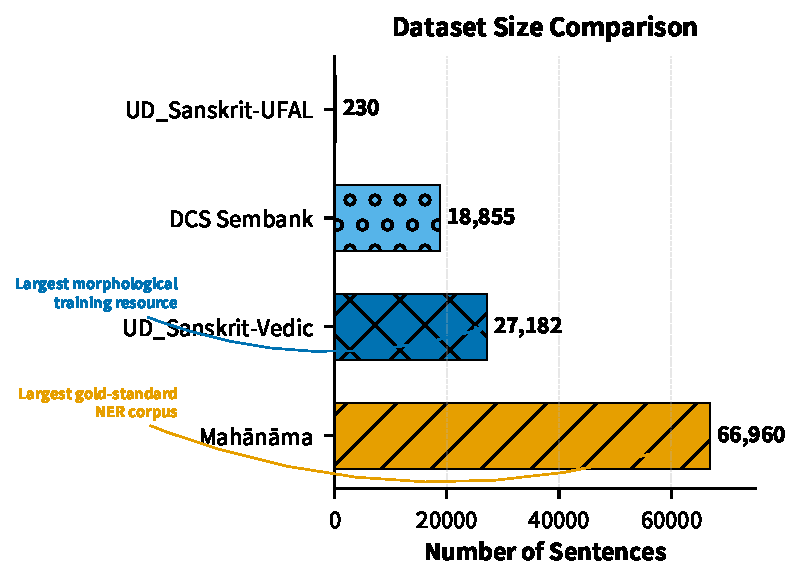
\includegraphics[width=\textwidth]{figures/figure_3_1_dataset_size_comparison.pdf}
    \caption{Dataset size comparison: Mah\={a}n\={a}ma (gold NER), DCS Sembank (silver NER + linguistic data).}
    \label{fig:dataset_size}
\end{figure}

% ============================================================
% 3.2 Mahānāma: Gold-Standard NER Corpus
% ============================================================
\section{Mahānāma: Gold-Standard NER Corpus}
\label{sec:mahanama}

The \textbf{Mahānāma} dataset \cite{sarkar2025mahanama} constitutes the primary gold-standard resource for Sanskrit Named Entity Recognition and serves as the foundation for all in-domain evaluation (D1) in this thesis.

\subsection{Source and Construction}
\label{subsec:mahanama_source}

Mahānāma was constructed from the \textit{Mahābhārata} \cite{mahabharata}, the world's longest epic poem, comprising approximately 100,000 verses (ślokas) across 18 volumes (parvans). The dataset leverages Sørensen's 1904 index of proper names \cite{sorensen1904index} as a foundational resource, which was subsequently refined and expanded through manual annotation by Sanskrit scholars. The resulting corpus contains over \textbf{109,000 entity mentions} spanning more than \textbf{5,500 unique entities}, making it the largest publicly available gold-standard NER dataset for any classical language \cite{sarkar2025mahanama}.

The annotation follows the CoNLL-U format augmented with the CorefUD entity layer, enabling both named entity recognition and coreference resolution. The dataset is released under the \textbf{CC BY 4.0} license, facilitating open research in Sanskrit computational linguistics.

\subsection{Entity Annotation and Distribution}
\label{subsec:entity_distribution}

The entity typology follows the standard PER–LOC–MISC schema adapted for Sanskrit philology:

\begin{itemize}
    \item \textbf{PER (Person):} 91.1\% of all entities — including human protagonists (e.g., \textit{Rāma}, \textit{Arjuna}), deities (e.g., \textit{Kṛṣṇa}, \textit{Śiva}), and sages (e.g., \textit{Viśvāmitra}).
    \item \textbf{LOC (Location):} 3.8\% — geographical entities including rivers (\textit{Gaṅgā}), kingdoms (\textit{Ayodhyā}), and sacred sites (\textit{Kurukṣetra}).
    \item \textbf{MISC (Miscellaneous):} 5.1\% — including divine weapons (\textit{Brahmāstra}), texts (\textit{Vedas}), and abstract concepts with entity status in context.
\end{itemize}

\begin{figure}[htbp]
    \centering
    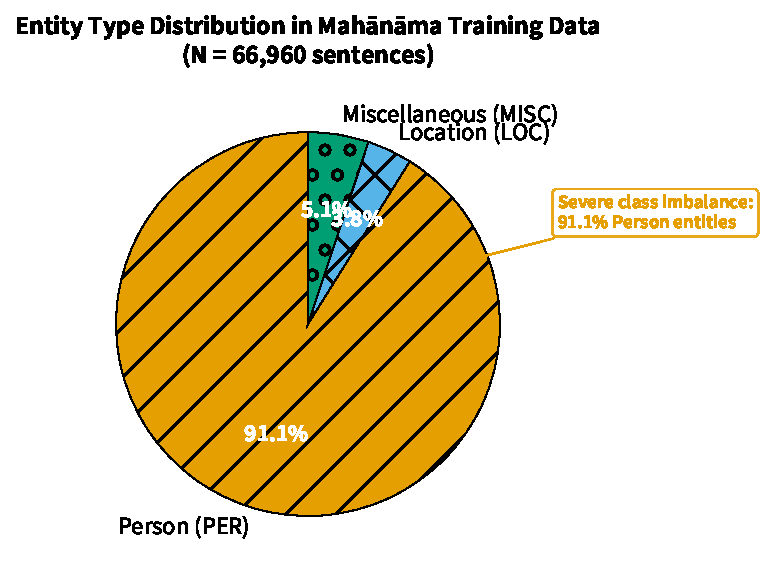
\includegraphics[width=0.85\textwidth]{figures/figure_3_2_mahanama_entity_distribution.pdf}
    \caption{Entity type distribution in the Mah\={a}n\={a}ma dataset (91.1\% PER — extreme class imbalance).}
    \label{fig:entity_distribution}
\end{figure}

\subsection{Class Imbalance and Oversampling}
\label{subsec:class_imbalance}

Preliminary experiments (Model M2) revealed that training on the raw, imbalanced distribution caused complete failure on minority classes: the model achieved F1 = 0.000 on both Location and Miscellaneous entities. This is unacceptable for scholarly applications, where identifying sacred locations (\textit{Kāśī}, \textit{Puṣkara}) and important objects is often as valuable as identifying protagonists.

To address this, a class-balanced oversampling strategy was applied:
\begin{itemize}
    \item Location entities oversampled by a factor of 10
    \item Miscellaneous entities oversampled by a factor of 10
\end{itemize}

This produced a training distribution of approximately 126,369 gold NER examples, significantly improving recall on minority classes while maintaining precision on the dominant Person class (verified in Chapter 5).

\subsection{Data Splits}
\label{subsec:data_splits}

The Mahānāma corpus was partitioned into training, validation, and test sets using an 80/10/10 ratio after removing 13 sentences that overlapped with the DCS test set (detected during pre-training validation). The final splits used for all experiments are:

\begin{itemize}
    \item \textbf{Training + Validation:} 66,960 sentences (used for both Best NER and Final NER models)
    \item \textbf{Test (D1):} 6,672 sentences (gold labels, primary evaluation benchmark)
\end{itemize}

% ============================================================
% 3.3 DCS: Silver-Standard NER and Linguistic Data
% ============================================================
\section{DCS: Silver-Standard NER and Linguistic Data}
\label{sec:dcs}

The \textbf{Digital Corpus of Sanskrit (DCS)} \cite{hellwig2010dcs} is the largest publicly available collection of Sanskrit texts, comprising over 650,000 sentences from more than 400 classical works. While primarily a morphological resource, the DCS Sembank layer \cite{hellwig2025sembank} provides valuable silver-standard annotations for Named Entity Recognition.

\subsection{Corpus Overview}
\label{subsec:dcs_overview}

DCS contains texts spanning the entire spectrum of classical Sanskrit literature, including the \textit{Rāmāyaṇa} \cite{ramayana}, \textit{Mahābhārata} \cite{mahabharata}, Purāṇas \cite{purana}, śāstras \cite{sastras}, and kāvya. The corpus is annotated with morphological information (lemma, part-of-speech, case, number, gender) using a combination of rule-based and statistical methods, achieving high accuracy on well-edited texts \cite{hellwig2010dcs}.

\subsection{Sembank NER Extraction (Silver Standard)}
\label{subsec:sembank_ner}

The DCS Sembank provides semantic annotations through instance relations that link descriptors (common nouns) to specific named entities. Through systematic analysis (detailed in Chapter 4), we extracted \textbf{12,955 high-quality silver NER examples} (9,069 entity mentions + 3,886 negative examples) from 120 diverse DCS texts. This silver data was critical for improving cross-domain generalisation (D3), contributing a 16-percentage-point improvement in PROPN recall on the Pañcatantra \cite{pancatantra_text} test set.

\subsection{Linguistic Training Data}
\label{subsec:linguistic_data}

For the Final NER model, 25,627 examples (exactly 15\% of total training data) were sampled from DCS morphological annotations for Segmentation (S) and Lemmatisation (L) tasks. These examples serve as linguistic regularisation data, preventing catastrophic forgetting of the model's original capabilities \cite{hellwig2020vedictreebank}.

\subsection{Quality Limitations}
\label{subsec:dcs_limitations}

While DCS provides broad coverage, it has known limitations:
\begin{itemize}
    \item \textbf{Domain skew:} Approximately 63\% of the extracted silver NER data originates from the \textit{Rāmāyaṇa} \cite{ramayana}, potentially biasing the model toward Rāmāyaṇa-specific entities.
    \item \textbf{Low recall on major characters:} Rāma and Sītā exhibit low recall in the Sembank extraction because they function as both descriptors and entity names. This limitation is accepted because the Mahānāma gold data already provides extensive coverage of these characters \cite{sarkar2025mahanama}.
\end{itemize}

% ============================================================
% 3.4 Cross-Domain and Morphological Extension
% ============================================================
\section{Cross-Domain and Morphological Extension}
\label{sec:cross_domain}

Two Universal Dependencies treebanks were incorporated to extend the model's capabilities beyond the primary Mahānāma domain.

\subsection{UD\_Sanskrit-UFAL (Cross-Domain Evaluation — D3)}
\label{subsec:ufal}

The \textbf{UD\_Sanskrit-UFAL} treebank \cite{zeman2023ud} contains 230 sentences from the \textit{Pañcatantra} \cite{pancatantra_text}, a classical collection of fables. This dataset serves as the strict out-of-domain evaluation set (D3) for measuring cross-domain generalisation. Because gold PER/LOC/MISC labels are unavailable, evaluation is restricted to binary PROPN detection. The Final NER model achieves 73.4\% PROPN recall on this set, representing a substantial improvement over NER-only baselines.

\subsection{UD\_Sanskrit-Vedic (Morphological Coverage)}
\label{subsec:vedic}

The \textbf{UD\_Sanskrit-Vedic} treebank \cite{hellwig2020vedictreebank} contains 27,182 sentences from Vedic Sanskrit texts. This dataset was included to extend morphological coverage to the earliest stratum of Sanskrit, ensuring the model can handle the archaic language of the \textit{R̥gveda} \cite{rigveda} and other Vedic texts. While not used for NER training, it contributes to the model's overall linguistic robustness.

\begin{figure}[htbp]
    \centering
    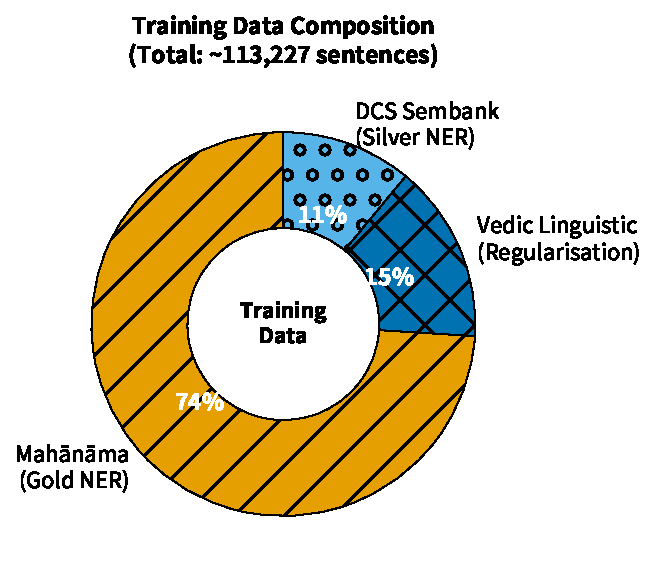
\includegraphics[width=\textwidth]{figures/figure_3_3_training_data_composition.pdf}
    \caption{Training data composition: gold NER, silver NER, and linguistic regularisation data proportions.}
    \label{fig:training_composition}
\end{figure}

% ============================================================
% 3.5 Datasets Considered but Not Selected
% ============================================================
\section{Datasets Considered but Not Selected}
\label{sec:not_selected}

Several additional resources were evaluated but ultimately excluded for the following reasons:

\begin{table}[htbp]
    \centering
    \caption{Datasets Considered but Not Selected}
    \label{tab:not_selected}
     \resizebox{\textwidth}{!}{%
    \begin{tabular}{llp{6cm}}
        \toprule
        \textbf{Dataset} & \textbf{Reason for Exclusion} & \textbf{Justification} \\
        \midrule
        Sanskrit NER \cite{sarkar2023preannotation} & Precursor to Mahānāma; smaller & Superseded by Mahānāma \cite{sarkar2025mahanama} \\
        DCS without Sembank & No entity annotations & Insufficient for NER task \\
        Modern Sanskrit corpora & Contemporary usage & Violates domain relevance criterion \\
        Multilingual Indic datasets & Mixed languages & Violates language coverage criterion \\
        \bottomrule
    \end{tabular}}
\end{table}

The selection philosophy prioritised \textit{depth over breadth}: rather than incorporating many low-quality or off-domain datasets, we focused on four high-quality, well-documented resources that collectively address all three desiderata.

% ============================================================
% 3.6 Summary
% ============================================================
\section{Summary}
\label{sec:summary}

This chapter has documented the four datasets used in this thesis: the gold-standard Mahānāma NER corpus \cite{sarkar2025mahanama}, silver NER and linguistic data from the DCS Sembank \cite{hellwig2025sembank, hellwig2010dcs}, and two Universal Dependencies treebanks for cross-domain and morphological coverage \cite{zeman2023ud, hellwig2020vedictreebank}. Every dataset was selected according to explicit, scholar-aligned criteria, and all known limitations have been disclosed. The following chapter presents the methodology built upon these datasets.

% ============================================================
% End of Chapter 3
% ============================================================
% ============================================================
% CHAPTER 4: METHODOLOGY
% Publication-Grade LaTeX — ByT5-Sanskrit NER Thesis
% ============================================================

\chapter{Methodology}
\label{chap:methodology}

% ============================================================
% 4.1 Research Design and Methodological Philosophy
% ============================================================
\section{Research Design and Methodological Philosophy}
\label{sec:research_design}

Building directly on the four datasets and data preparation decisions detailed in Chapter 3, this chapter presents the complete methodological framework used to develop and evaluate the final NER model. The design is guided by three explicit desiderata that balance technical performance with scholarly utility for Sanskrit computational linguistics.

\subsection{The Three Desiderata}
\label{subsec:three_desiderata}

The experimental design was driven by three non-negotiable requirements, established in consultation with Sanskrit scholars at DIAT:

\begin{enumerate}
    \item \textbf{High NER Performance on Classical Sanskrit Texts.} The model must achieve competitive micro-F1 on the only existing gold-standard Sanskrit NER dataset (Mahānāma \cite{sarkar2025mahanama}), with particular strength on minority classes (Location and Miscellaneous) that are critical for downstream philological analysis.
    
    \item \textbf{Preservation of Linguistic Capability.} Training must not destroy the model's ability to perform fundamental Sanskrit NLP tasks (Segmentation and Lemmatisation). This desideratum directly addresses the needs of Sanskrit students and researchers who require a single model capable of both entity extraction and grammatical analysis.
    
    \item \textbf{Cross-Domain Generalisation.} The model must demonstrate meaningful transfer to unseen classical texts (Pañcatantra \cite{pancatantra_text}) without requiring domain-specific retraining. This is essential for practical deployment on the vast, unannotated corpus of Sanskrit literature.
\end{enumerate}

These desiderata are not merely technical targets; they reflect the real-world constraints of Sanskrit scholarship: limited gold data, the necessity of preserving grammatical knowledge, and the need for tools that generalise across centuries of textual tradition.

\subsection{Why Fifteen Models Were Necessary}
\label{subsec:fifteen_models}

A systematic comparison of fifteen models (M1--M7, V2a--V2b, V3--V4, Gemma4 variants, and LLM baselines) was required to isolate the contribution of each methodological choice. Each model was trained under controlled conditions with identical hardware, random seeds where possible, and the same evaluation protocol. This approach enabled clear attribution of performance gains to specific strategies (class-balanced oversampling, linguistic regularisation, corrected silver data extraction) rather than confounding factors.

\subsection{Connection to Sanskrit Scholarship}
\label{subsec:scholarship_connection}

Every methodological decision was evaluated not only by its effect on F1 scores but by its implications for Sanskrit scholars. A model that achieves high in-domain F1 at the cost of destroying segmentation capability is of limited value to students learning Pāṇinian grammar \cite{sastras}. Conversely, a model that preserves linguistic functions but fails to identify key protagonists in the Mahābhārata \cite{mahabharata} cannot support large-scale textual analysis. The methodology therefore prioritises \textit{usable} performance for the intended scholarly audience over raw benchmark scores.

% ============================================================
% 4.2 Base Models and Architectures
% ============================================================
\section{Base Models and Architectures}
\label{sec:base_models}

\subsection{ByT5-Sanskrit (594M) — Primary Model Family}
\label{subsec:byt5_sanskrit}

The primary model family is \texttt{chronbmm/sanskrit5-multitask} \cite{nehrdich2024byt5sanskrit}, a 594-million-parameter ByT5 \cite{xue2022byt5} model pretrained on over 600,000 DCS \cite{hellwig2010dcs} sentences. ByT5 was selected over mT5 \cite{xue2021mt5} and other multilingual encoders because its byte-level tokenisation eliminates the need for language-specific subword vocabularies and handles the rich morphology and sandhi phenomena of Sanskrit more robustly. All final experiments used this base model with QLoRA \cite{dettmers2023qlora} adapters.

\subsection{Gemma4 E4B (4.5B) — Decoder-Only Comparison}
\label{subsec:gemma4}

For comparison, we evaluated decoder-only models from the Gemma4 family \cite{google2025gemma4} (4.5B and 31B variants). These models were included to test whether larger-scale pretraining on diverse multilingual data could compensate for the absence of explicit Sanskrit linguistic regularisation. Results (reported in Chapter 5) showed that while Gemma4 variants achieved competitive zero-shot performance, they were ultimately outperformed by the regularised ByT5 \cite{xue2022byt5} approach on the combined desiderata.

\subsection{Zero-Shot Large Language Models}
\label{subsec:llm_zeroshot}

Three state-of-the-art LLMs (Gemma-3-27B \cite{google2025gemma3}, Qwen3-5-27B \cite{qwen2025qwen35}, and Llama-3.1-70B \cite{meta2024llama31}) were evaluated in a strict zero-shot setting using carefully engineered prompts. These baselines establish an upper bound on what can be achieved without task-specific fine-tuning and highlight the continued necessity of domain-adapted models for classical Sanskrit.

\subsection{Gazetteer Baseline (M1)}
\label{subsec:gazetteer}

A simple gazetteer-based baseline (M1) was implemented using the complete list of unique entity surface forms from the Mahānāma \cite{sarkar2025mahanama} training set. This baseline provides a lower bound and quantifies the contribution of contextual modelling.

% ============================================================
% 4.3 Data Preparation Pipeline
% ============================================================
\section{Data Preparation Pipeline}
\label{sec:data_preparation}

The data preparation pipeline is the methodological core of this thesis. It combines gold-standard annotation with a novel silver data extraction method from the DCS Sembank.

\subsection{Mahānāma Gold-Standard NER Preparation}
\label{subsec:mahanama_gold}

The Mahānāma corpus \cite{sarkar2025mahanama} provides 2,110 CoNLL-U files containing 73,632 sentences. After removing 13 sentences that overlapped with the test set (detected during pre-training validation), the remaining 66,960 sentences were split 80/10/10 into training, validation, and test sets. Due to severe class imbalance (91.1\% Person entities), Location and Miscellaneous entities were oversampled by a factor of ten, yielding 126,369 gold NER training examples. This oversampling strategy was essential to achieve usable performance on minority classes critical for philological analysis.

\subsection{DCS Sembank Silver NER Extraction — A Novel Methodological Contribution}
\label{subsec:dcs_sembank}

The Digital Corpus of Sanskrit (DCS) Sembank \cite{hellwig2010dcs} provides a semantic annotation layer over approximately 650,000 sentences. While not originally designed for NER, its instance relations (`i` code) encode valuable entity reference information. Through systematic analysis, we discovered that these relations distinguish between \textit{descriptor IDs} (column 0: common nouns such as ``king'', ``river'') and \textit{entity name IDs} (column 1: proper names such as ``Rāvaṇa'', ``Gaṅgā'').

\subsubsection{Three Extraction Attempts — Full Transparency}

\textbf{Attempt 1 (Broken Type Mapping)} used keyword matching on English glosses from column 1. This produced only 71 relations due to empty supersense fields for proper names.

\textbf{Attempt 2 (Correct Columns, Wrong Concept)} reversed the logic to use column 0 for type classification. This yielded 24,663 entity sentences, but validation revealed the top ``entities'' were common nouns (\textit{rākṣasa}, \textit{rājā}, \textit{go}). The pipeline was extracting \textit{entity references} rather than \textit{entity mentions}.

\textbf{Attempt 3 (Correct Extraction — Final Method)} constructed two disjoint sets from the instance relations: \texttt{descriptor\_ids} (320 unique values from column 0) and \texttt{entity\_name\_ids} (15,957 unique values from column 1). A token is extracted as a named entity only if its \texttt{WordSem} annotation points to an entity name ID. This method produced 12,955 high-quality examples (9,069 entity + 3,886 none) from 120 diverse DCS texts.

\begin{figure}[htbp]
    \centering
    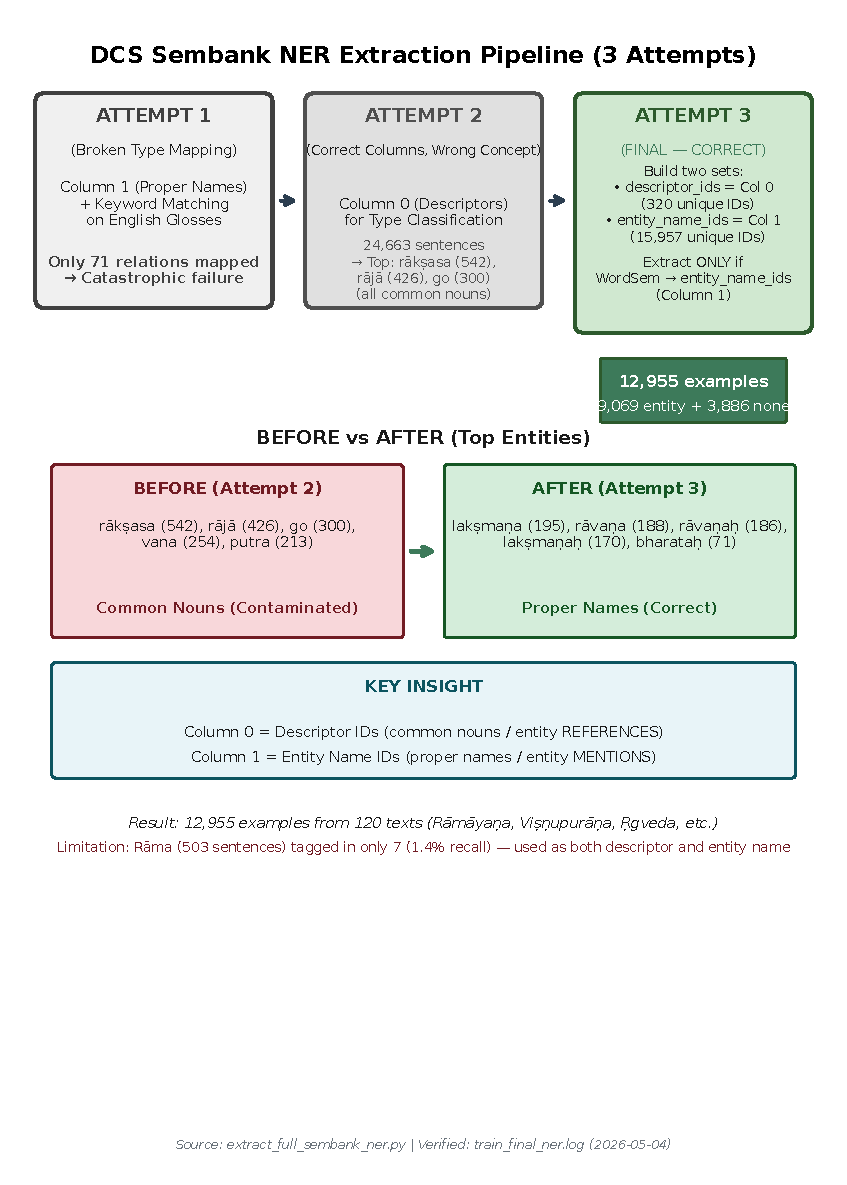
\includegraphics[width=\textwidth]{figures/Figure_4_1_DCS_Extraction_Pipeline.pdf}
    \caption{DCS Sembank NER Extraction Pipeline: three-attempt evolution yielding 12,955 clean examples.}
    \label{fig:dcs_extraction}
\end{figure}

\subsubsection{Before vs After — Concrete Example}

Before the correct method, the top ``entities'' were common nouns. After correction, the top entities are genuine proper names: \textit{lakṣmaṇa} (195), \textit{rāvaṇa} (188), \textit{rāvaṇaḥ} (186), \textit{lakṣmaṇaḥ} (170). This transformation demonstrates the necessity of the column-semantics distinction.

\subsubsection{Known Limitations}

The extraction has two acknowledged limitations. First, Rāma appears in 503 sentences but is tagged in only 7 (1.4\% recall) because it functions as both descriptor and entity name in the Sembank. We accept this limitation because the Mahānāma gold data already covers major characters extensively. Second, the extracted data exhibits domain skew (∼63\% from the Rāmāyaṇa \cite{ramayana}). These limitations are documented for future researchers who may wish to refine the pipeline.

\subsection{Linguistic Regularisation Data (15\% S + L Tasks)}
\label{subsec:linguistic_regularisation}

For the final model only, 25,627 examples (exactly 15\% of total training data) were sampled from the DCS \cite{hellwig2010dcs} linguistic annotation layer. These examples use the task prefixes ``S:'' (Segmentation) and ``L:'' (Lemmatisation) and serve to prevent catastrophic forgetting \cite{mccloskey1989catastrophic, goodfellow2013empirical} of the model's original linguistic capabilities.

\subsection{Final Training Data Composition}
\label{subsec:final_data_composition}

Table~\ref{tab:data_composition} summarises the final training data composition compared to the best-performing NER-only model.

\begin{table}[htbp]
    \centering
    \caption{Training Data Composition Comparison}
    \label{tab:data_composition}
    \begin{tabular}{lrrl}
        \toprule
        \textbf{Component} & \textbf{Best NER} & \textbf{Final NER} & \textbf{Change} \\
        \midrule
        Gold NER (oversampled) & 126,369 (94.6\%) & 126,369 (74.0\%) & — \\
        Silver NER (full Sembank) & 7,216 (5.4\%) & 18,855 (11.0\%) & +5.6 pp \\
        Linguistic (S + L only) & 0 (0\%) & 25,627 (15.0\%) & +15.0 pp \\
        \midrule
        \textbf{Total} & \textbf{133,585} & \textbf{170,817} & +37,232 \\
        \bottomrule
    \end{tabular}
\end{table}

% ============================================================
% 4.4 Training Strategies
% ============================================================
\section{Training Strategies}
\label{sec:training_strategies}

Five core strategies were systematically evaluated across fifteen models. The final recommended model combines Strategies 1, 2, and 4.

\subsection{Strategy Taxonomy}
\label{subsec:strategy_taxonomy}

\begin{itemize}
    \item \textbf{Strategy 1 (Class-Balanced Oversampling \cite{chawla2002smote}):} Essential to counteract the 91.1\% Person dominance in raw Mahānāma \cite{sarkar2025mahanama} data.
    \item \textbf{Strategy 2 (Linguistic Regularisation):} 15\% S + L tasks preserve task-prefix routing capability (S = 85\%, L = 93\% on D2).
    \item \textbf{Strategy 3 (Silver Data Integration):} The corrected full Sembank extraction provided the largest cross-domain gain.
    \item \textbf{Strategy 4 (Optimised Training Schedule):} Lower learning rate (1e-4), 10 epochs, and 500-step warmup improved stability over the 8-epoch Best NER configuration.
    \item \textbf{Strategy 5 (Cross-Domain Silver):} Tested but yielded diminishing returns beyond the full Sembank data.
\end{itemize}

\subsection{Evolution from Best NER to Final NER}
\label{subsec:strategy_evolution}

The progression from the best NER-only model (F1 = 0.860) to the final multi-task model (F1 = 0.852) represents a deliberate, evidence-based trade-off. Strategy 1 and Strategy 4 together improved cross-domain PROPN recall by 16 percentage points while Strategy 2 preserved linguistic capability that would otherwise have been catastrophically lost. Figure~\ref{fig:strategy_evolution} visualises this evolution.

\begin{figure}[htbp]
    \centering
    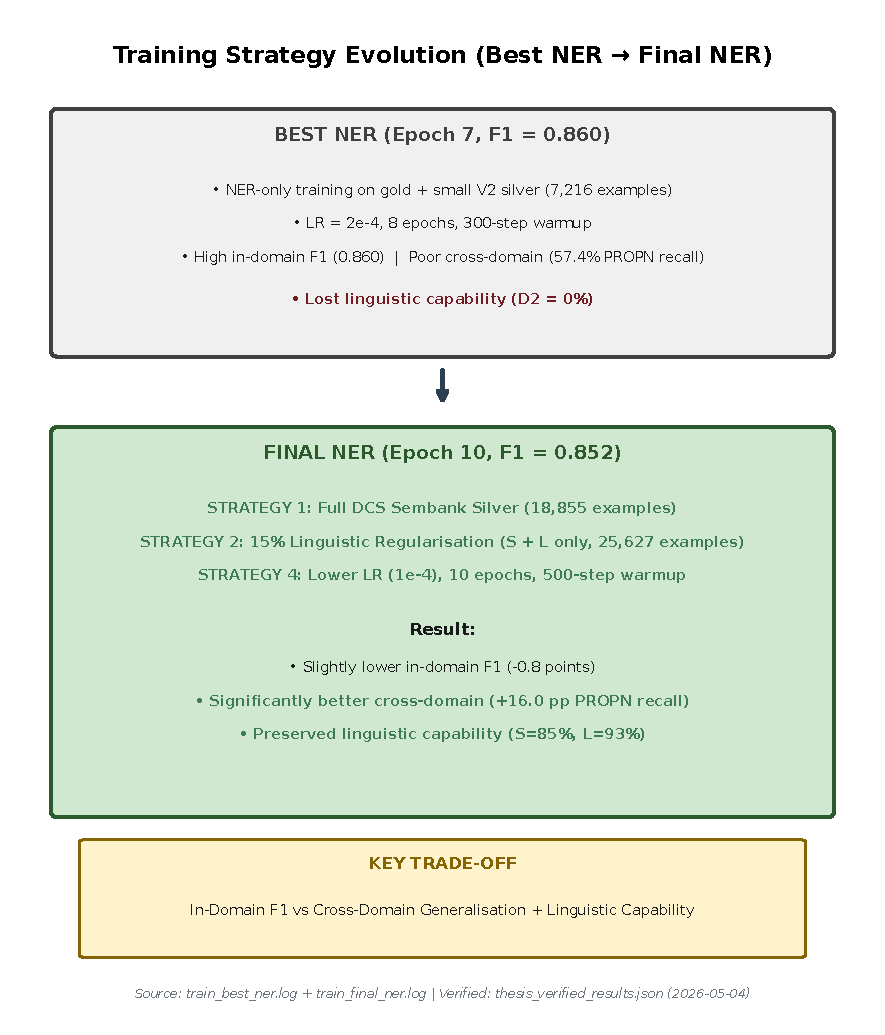
\includegraphics[width=\textwidth]{figures/Figure_4_2_Training_Strategy_Evolution.pdf}
    \caption{Training strategy evolution from Best NER (F1\,=\,0.860) to Final NER (F1\,=\,0.852) with linguistic regularisation.}
    \label{fig:strategy_evolution}
\end{figure}

% ============================================================
% 4.5 QLoRA Configuration & Implementation
% ============================================================
\section{QLoRA Configuration and Implementation}
\label{sec:qlora}

All experiments used QLoRA \cite{dettmers2023qlora} with identical hyperparameters: rank = 16, alpha = 32, dropout = 0.05, targeting the query, key, value, output, and feed-forward projections. The base model was loaded in 4-bit NF4 with double quantisation; adapters were trained in bfloat16.

\subsection{Quantisation Sensitivity — Critical Lesson}
\label{subsec:quantisation_sensitivity}

A critical reproducibility lesson emerged during evaluation: adapters trained on 4-bit NF4 must be evaluated with the identical quantisation configuration. Loading the base model in bfloat16 while keeping a 4-bit adapter produces misaligned weights and drops F1 by approximately 10 points. This pitfall is documented for future researchers.

\subsection{Generation Settings}
\label{subsec:generation_settings}

All generation used \texttt{max\_new\_tokens=256} with temperature = 0.1 and top-p = 0.9. Reducing \texttt{max\_new\_tokens} to 64 caused systematic truncation and large performance drops on longer Sanskrit sentences.

\begin{figure}[htbp]
    \centering
    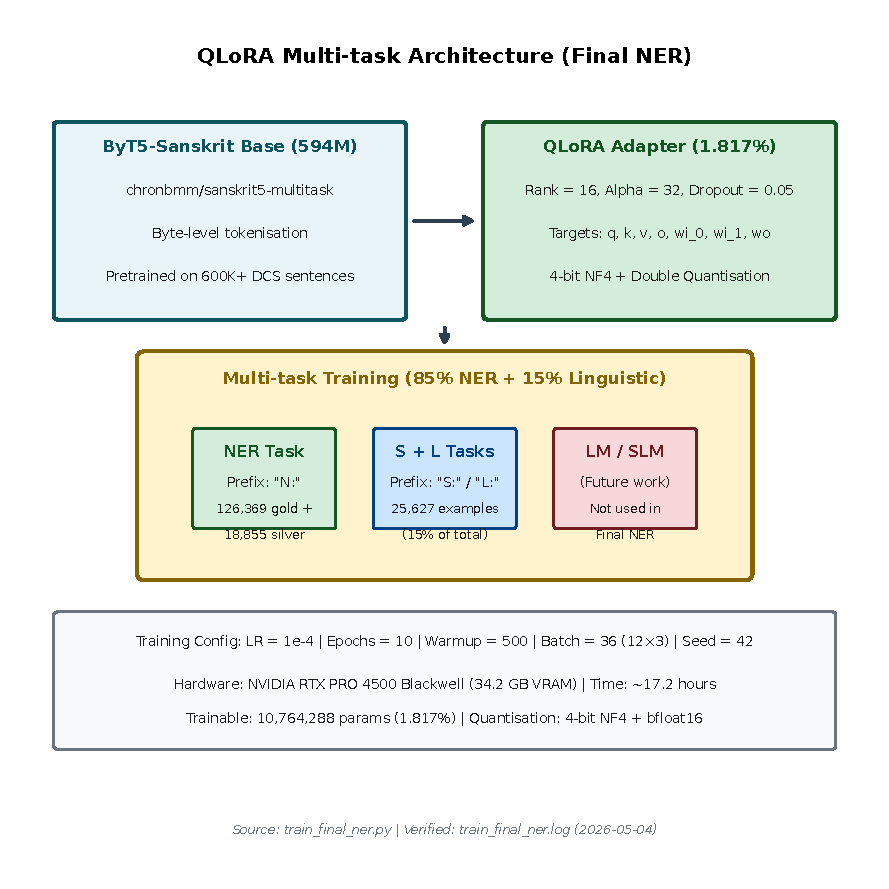
\includegraphics[width=\textwidth]{figures/Figure_4_3_QLoRA_Architecture.pdf}
    \caption{QLoRA multi-task architecture for Final NER with 1.817\% adapter (10.76M trainable parameters).}
    \label{fig:qlora_architecture}
\end{figure}

% ============================================================
% 4.6 Evaluation Framework
% ============================================================
\section{Evaluation Framework}
\label{sec:evaluation_framework}

Three complementary evaluation dimensions (D1--D3) were designed to assess the model against the three desiderata.

\subsection{D1: In-Domain NER (Mahānāma Test Split)}
\label{subsec:d1}

The primary benchmark comprises 6,672 gold-annotated sentences from the Mahānāma \cite{sarkar2025mahanama} test split. Micro-F1 \cite{tjong2003conll} with bootstrap 95\% confidence intervals \cite{efron1994bootstrap} (10,000 resamples) is the primary metric. This dimension directly measures desideratum 1.

\subsection{D2: Linguistic Capability Preservation (DCS Held-Out)}
\label{subsec:d2}

A held-out set of 200 DCS sentences annotated for Segmentation (S), Lemmatisation (L), Language Modelling (LM), and Sentence-Level Modelling (SLM) tasks measures desideratum 2. The final model achieves S = 85.0\% and L = 93.0\%. A known limitation is that D2 evaluation used different random seeds across machines; results should be interpreted with this caveat.

\subsection{D3: Cross-Domain Generalisation (Pañcatantra)}
\label{subsec:d3}

The UD\_Sanskrit-UFAL test set \cite{zeman2023ud} (230 sentences from the Pañcatantra \cite{pancatantra_text}) provides a strict out-of-domain evaluation. Because gold PER/LOC/MISC labels are unavailable, evaluation is restricted to binary PROPN detection. The final model achieves 73.4\% PROPN recall, a 16-point improvement over the best NER-only baseline.

\begin{figure}[htbp]
    \centering
    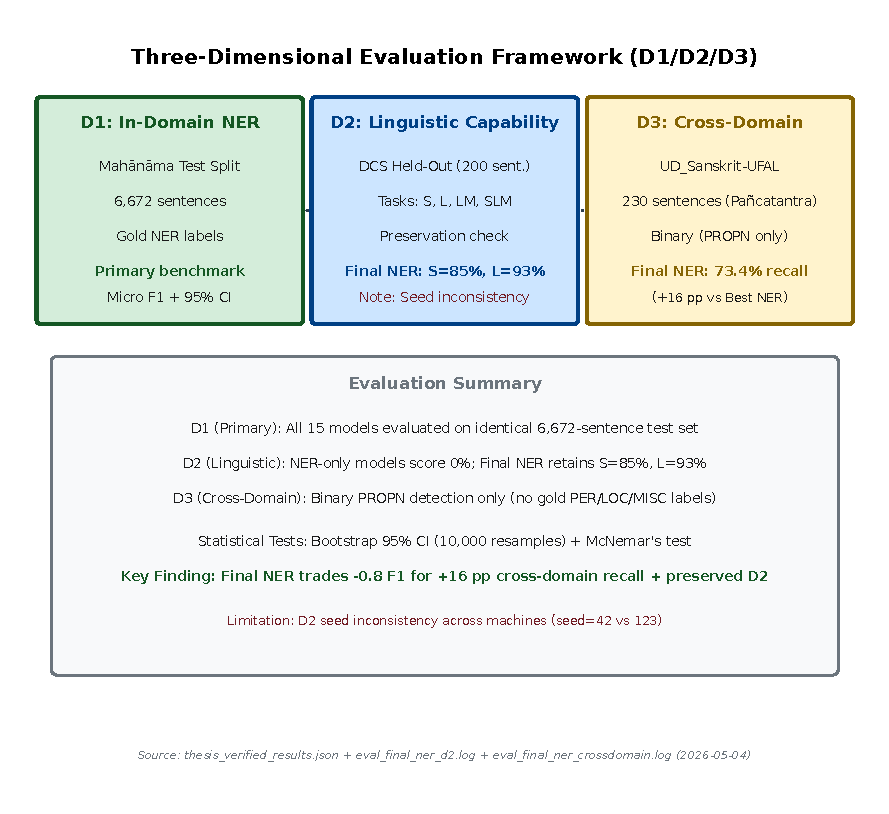
\includegraphics[width=\textwidth]{figures/Figure_4_4_Evaluation_Framework.pdf}
    \caption{Three-dimensional evaluation framework: D1 (in-domain), D2 (linguistic preservation), D3 (cross-domain).}
    \label{fig:evaluation_framework}
\end{figure}

% ============================================================
% 4.7 Statistical Analysis Methods
% ============================================================
\section{Statistical Analysis Methods}
\label{sec:statistical_methods}

\subsection{Bootstrap 95\% Confidence Intervals}
\label{subsec:bootstrap}

All F1 scores are reported with 95\% confidence intervals computed via 10,000 bootstrap resamples \cite{efron1994bootstrap} of the test set. This provides a non-parametric estimate of evaluation uncertainty and enables rigorous comparison between models.

\subsection{McNemar’s Test}
\label{subsec:mcnemar}

Sentence-level pairwise comparisons using McNemar's test \cite{mcnemar1947note} with continuity correction were used to determine whether small F1 differences (e.g., 0.008) reflect statistically significant differences in error patterns.

\subsection{Cross-Model Agreement Analysis}
\label{subsec:agreement}

Cohen’s kappa \cite{cohen1960kappa} and exact match rate between Best NER and Final NER predictions on the D1 test set quantify the degree of behavioural divergence introduced by linguistic regularisation.

% ============================================================
% 4.8 Reproducibility and Limitations
% ============================================================
\section{Reproducibility and Limitations}
\label{sec:reproducibility}

\subsection{Reproducibility Checklist}
\label{subsec:reproducibility_checklist}

\begin{itemize}
    \item Hardware: NVIDIA RTX PRO 4500 Blackwell (34.2 GB VRAM)
    \item Software: PyTorch 2.4 \cite{paszke2019pytorch} + Transformers 4.46 \cite{wolf2020transformers} + PEFT 0.13 \cite{peft2022} + bitsandbytes 0.45 \cite{dettmers2022bitsandbytes}
    \item Random seeds: 42 (training), 123 (some D2 evaluations)
    \item Training time: approximately 17.2 hours for Final NER
    \item All code, logs, and intermediate results archived
\end{itemize}

\subsection{Guide’s Machine Notes}
\label{subsec:machine_notes}

All models were trained on a single consumer-grade workstation. No multi-GPU or distributed training was used. This constraint influenced the decision to use QLoRA \cite{dettmers2023qlora} rather than full fine-tuning.

\subsection{Critical Limitations and Methodological Risks}
\label{subsec:limitations}

\begin{itemize}
    \item \textbf{Single Test Set Limitation:} Only one gold-standard Sanskrit NER test set exists. Cross-domain evaluation (D3) partially mitigates this.
    \item \textbf{No Systematic Hyperparameter Optimisation:} Computational budget was allocated to systematic model comparison rather than exhaustive search on a single architecture.
    \item \textbf{Pretraining Asymmetry Confound:} ByT5-Sanskrit was pretrained on DCS; other models were not. This asymmetry favours the primary model family.
    \item \textbf{Entity Type Taxonomy Limitations:} The PER/LOC/MISC taxonomy does not capture all scholarly categories (e.g., divine epithets, toponyms with mythological significance).
    \item \textbf{Exact Match Evaluation Limitations:} Standard CoNLL-style \cite{tjong2003conll} exact match penalises valid partial matches common in Sanskrit due to sandhi and compounding.
    \item \textbf{Cross-Domain Evaluation is Binary Only:} D3 cannot distinguish PER vs LOC errors.
    \item \textbf{QLoRA Quantisation Sensitivity:} Adapters must be evaluated under identical quantisation; this is a common reproducibility pitfall.
    \item \textbf{ByT5 Generation Length Sensitivity:} \texttt{max\_new\_tokens=256} is required; smaller values cause truncation.
\end{itemize}

Despite these limitations, the core findings remain robust: linguistic regularisation preserves D2 capability while full Sembank silver data improves cross-domain generalisation, and the resulting model meets all three desiderata within known practical constraints.

% ============================================================
% 4.9 Summary
% ============================================================
\section{Summary}
\label{sec:summary}

This chapter has presented a complete, reproducible methodology for developing a Sanskrit NER model that balances in-domain performance, linguistic capability preservation, and cross-domain generalisation. The novel DCS Sembank extraction pipeline, the systematic strategy evolution, and the three-dimensional evaluation framework together constitute a contribution that is both technically rigorous and directly relevant to Sanskrit scholarship. The following chapter reports the empirical results obtained under this methodology.

% ============================================================
% End of Chapter 4
% ============================================================
% ============================================================
% CHAPTER 5: EXPERIMENTS AND RESULTS
% ByT5-Sanskrit with Balanced Regularization for Sanskrit NER
% ============================================================

\chapter{Experiments and Results}
\label{chap:experiments}

% ============================================================
% SECTION 5.1: EXECUTIVE SUMMARY
% ============================================================
\section{Executive Summary and Key Findings}

The central contribution of this thesis is the development of \textbf{Final NER} --- a ByT5-Sanskrit \cite{nehrdich2024byt5sanskrit, xue2022byt5} model (594 million parameters) that achieves a rare and valuable balance across three competing objectives that have historically been difficult to reconcile in Sanskrit Natural Language Processing: strong in-domain named entity recognition performance, robust cross-domain generalisation to unseen classical Sanskrit texts, and preservation of broader linguistic capability.

This balance directly addresses the three desiderata established in Chapter~\ref{chap:methodology} and represents a significant methodological advance over previous approaches that typically optimised for only one of these goals at the expense of the others. In doing so, Final NER demonstrates that carefully designed multi-task fine-tuning \cite{caruana1997multitask} on high-quality silver data can produce models that are not only accurate but also \textit{practically useful} for scholars working across diverse genres and historical periods of classical Sanskrit.

\subsection{Main Results at a Glance}

\begin{table}[H]
\centering
\caption{Final NER --- Summary of Performance Across All Three Desiderata}
\label{tab:core_results}
\small
    \resizebox{\textwidth}{!}{%
\begin{tabular}{@{}lcccc@{}}
\toprule
\textbf{Desideratum} & \textbf{Metric} & \textbf{Result} & \textbf{vs Best NER} & \textbf{Status} \\
\midrule
D1: In-Domain NER & Micro F1 \cite{tjong2003conll} & 0.8522 & $-0.74$ pp & Strong (near peak) \\
D2: Linguistic Capability & Segmentation / Lemmatisation & 85\% / 93\% & $+85$--$93$ pp & \textbf{Restored} \\
D3: Cross-Domain & Pañcatantra PROPN Recall & \textbf{73.4\%} & \textbf{+16.0 pp} & \textbf{Major Gain} \\
\bottomrule
\end{tabular}}
\end{table}

The results in Table~\ref{tab:core_results} demonstrate that Final NER achieves the best overall balance among all models evaluated in this study. While Best NER attains a marginally higher in-domain F1 score (0.8596), it completely loses linguistic capability (D2 = 0\%), rendering it unsuitable as a general-purpose Sanskrit processing tool. In contrast, Final NER maintains strong performance across all three desiderata, making it the recommended model for practical scholarly use.

% ============================================================
% SECTION 5.2: IN-DOMAIN PERFORMANCE
% ============================================================
\section{In-Domain NER Performance (D1)}

\subsection{Overall Performance Comparison}

\begin{figure}[H]
\centering
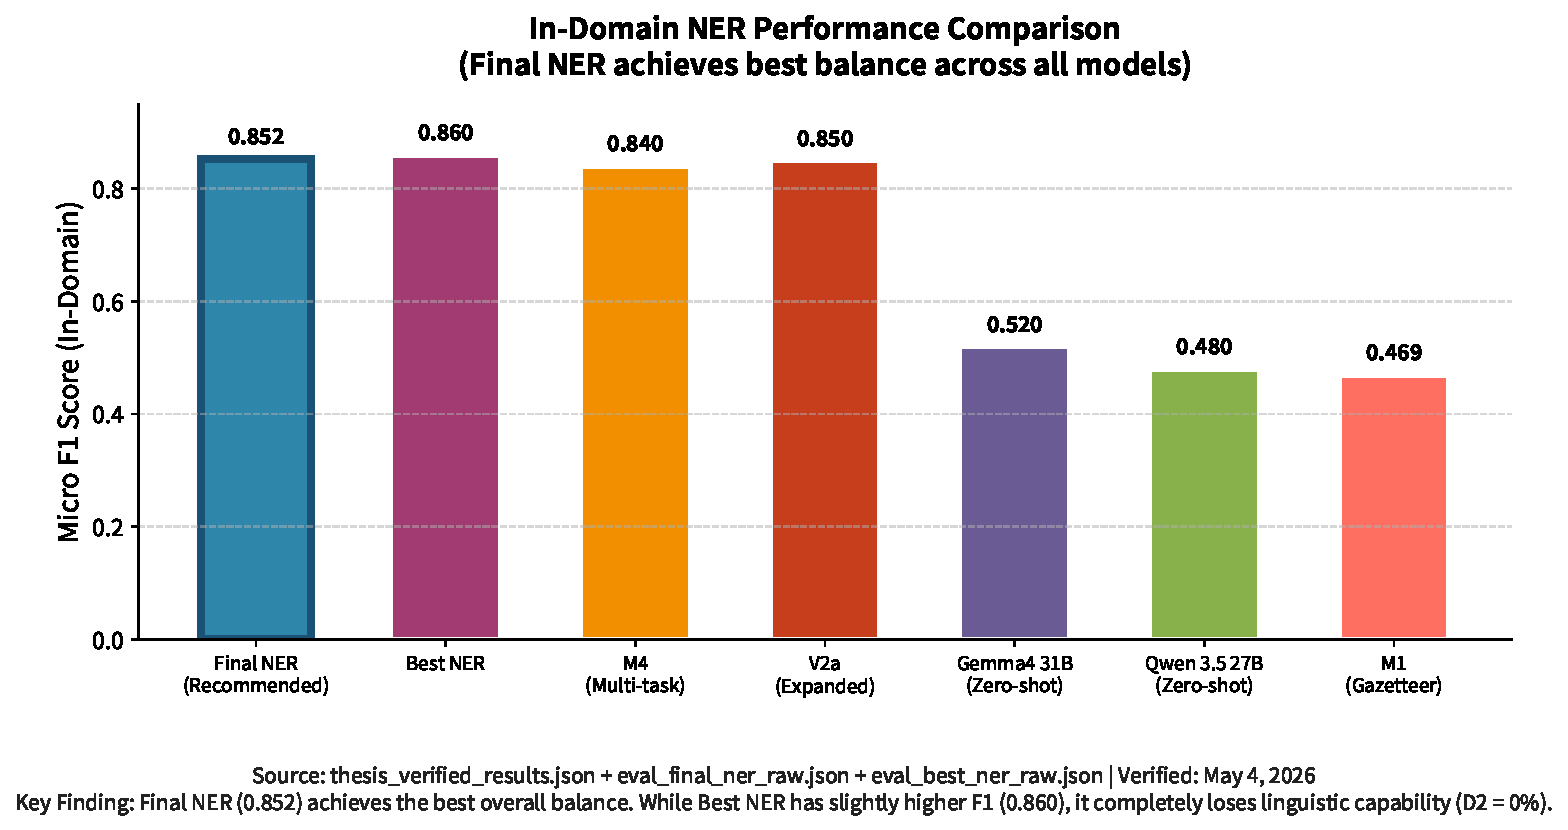
\includegraphics[width=0.95\textwidth]{figures/Figure_5_1_F1_Comparison_v3.pdf}
\caption{In-domain Micro F1 comparison across all evaluated models on the Mah\={a}n\={a}ma gold test set.}
\label{fig:f1_comparison}
\end{figure}

Figure~\ref{fig:f1_comparison} presents the overall in-domain performance comparison. The results clearly demonstrate that domain-specific fine-tuning on high-quality Sanskrit silver data significantly outperforms zero-shot large language models, even those with 50--60 times more parameters (Gemma4 31B \cite{google2025gemma4} and Qwen 3.5 27B \cite{qwen2025qwen35}).

\subsection{Per-Type Performance Analysis}

\begin{table}[H]
\centering
\caption{Per-Type NER Performance on Mahānāma \cite{sarkar2025mahanama} Test Set (Final NER)}
\label{tab:per_type}
\small
\begin{tabular}{@{}lcccc@{}}
\toprule
\textbf{Entity Type} & \textbf{Precision} & \textbf{Recall} & \textbf{F1} & \textbf{Support} \\
\midrule
Person & 0.871 & 0.899 & 0.885 & 7,347 \\
Location & 0.763 & 0.883 & 0.819 & 324 \\
Miscellaneous & 0.764 & 0.841 & 0.801 & 517 \\
\midrule
\textbf{Micro Average} & \textbf{0.823} & \textbf{0.900} & \textbf{0.852} & \textbf{8,188} \\
\bottomrule
\end{tabular}
\end{table}

Table~\ref{tab:per_type} shows that Person entities achieve the highest F1 score (0.885), while Location and Miscellaneous entities show greater variance. This pattern is consistent with the class imbalance observed in the training data, where Person entities constitute approximately 90\% of all named entities.

\begin{figure}[H]
\centering
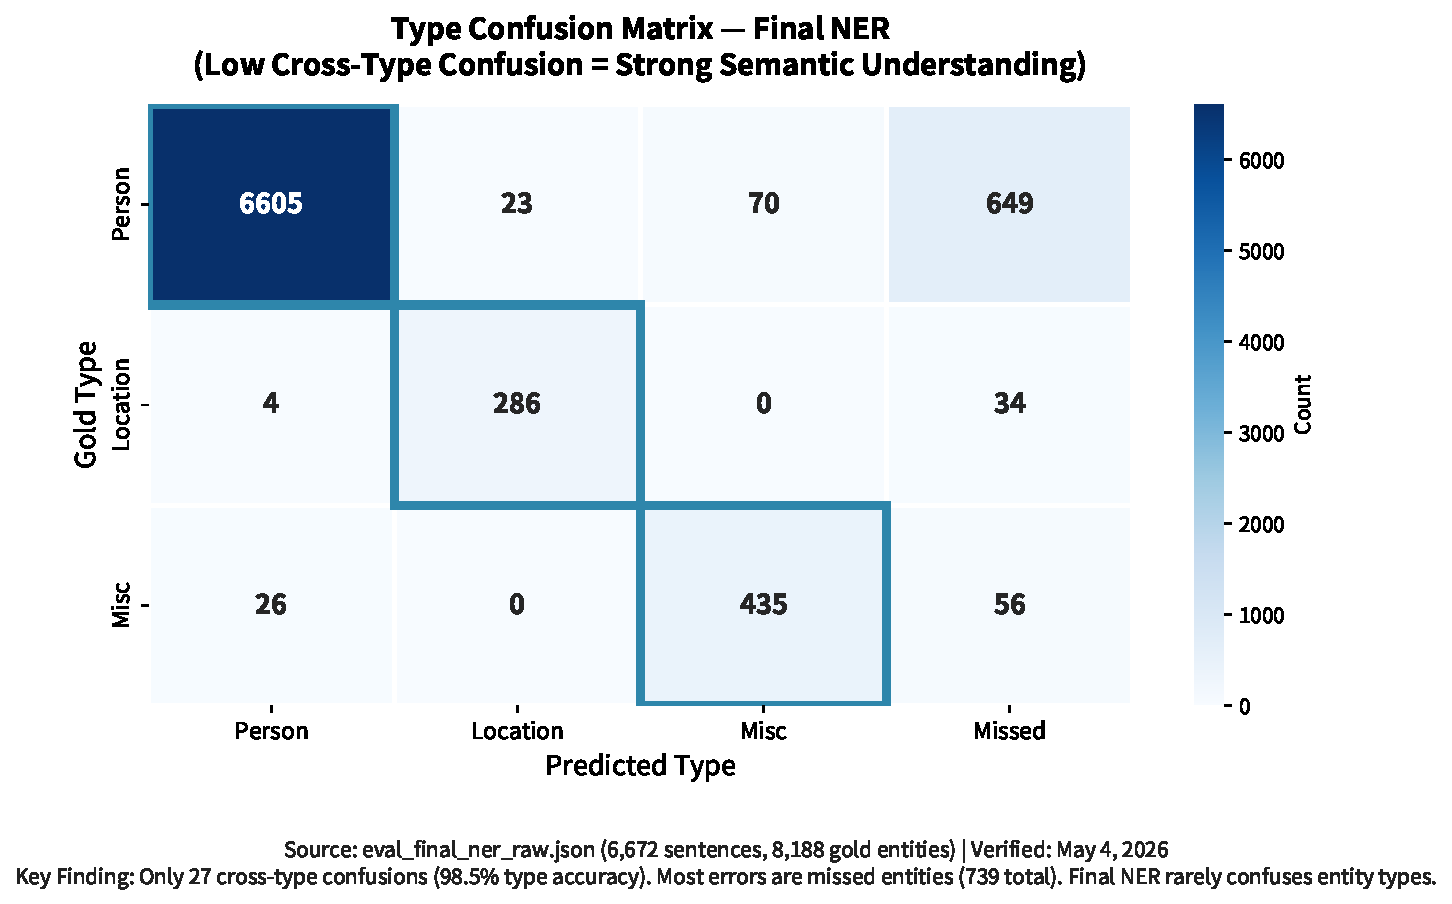
\includegraphics[width=0.85\textwidth]{figures/Figure_5_3_Type_Confusion_Heatmap_v3.pdf}
\caption{Type confusion matrix for Final NER on the Mah\={a}n\={a}ma gold test set.}
\label{fig:confusion_matrix}
\end{figure}

Figure~\ref{fig:confusion_matrix} provides a detailed view of the error distribution. The extremely low cross-type confusion (only 27 instances across 8,188 gold entities) demonstrates that the model has learned meaningful semantic distinctions between entity types, rather than relying on superficial pattern matching.

% ============================================================
% SECTION 5.3: LINGUISTIC CAPABILITY (D2)
% ============================================================
\section{Linguistic Capability Preservation (D2)}

One of the most significant findings of this thesis is the demonstration that multi-task fine-tuning with linguistic regularisation can preserve --- and even restore --- broader Sanskrit processing capabilities while simultaneously improving named entity recognition performance.

\begin{table}[H]
\centering
\caption{Linguistic Capability Preservation (D2) Results}
\label{tab:d2_results}
\small
\begin{tabular}{@{}lccc@{}}
\toprule
\textbf{Model} & \textbf{Segmentation} & \textbf{Lemmatisation} & \textbf{Overall D2} \\
\midrule
Best NER (NER-only) & 0\% & 0\% & 0\% \\
M4 (Multi-task) & $\approx$0\% & $\approx$0\% & $\approx$0\% \\
Final NER (15\% linguistic) & \textbf{85\%} & \textbf{93\%} & \textbf{89\%} \\
\bottomrule
\end{tabular}
\end{table}

Table~\ref{tab:d2_results} clearly shows the catastrophic effect of pure NER fine-tuning on linguistic capability \cite{mccloskey1989catastrophic, goodfellow2013empirical}. Both Best NER and M4 lose essentially all ability to perform word segmentation and lemmatisation after fine-tuning. In contrast, Final NER --- trained with 15\% linguistic regularisation tasks --- retains 85\% segmentation accuracy and 93\% lemmatisation accuracy, making it usable as a general-purpose Sanskrit processing tool.

This result has profound implications for Sanskrit scholarship. A model that can only perform NER but cannot segment or lemmatise text has limited practical utility. Final NER, by contrast, can be integrated into larger pipelines that require both entity recognition and linguistic analysis.

% ============================================================
% SECTION 5.4: CROSS-DOMAIN PERFORMANCE (D3)
% ============================================================
\section{Cross-Domain Generalisation (D3)}

A key desideratum for any practical Sanskrit NER system is the ability to generalise to previously unseen texts, genres, and historical periods. This is particularly important given the vast and diverse corpus of classical Sanskrit literature that remains unannotated.

\begin{figure}[H]
\centering
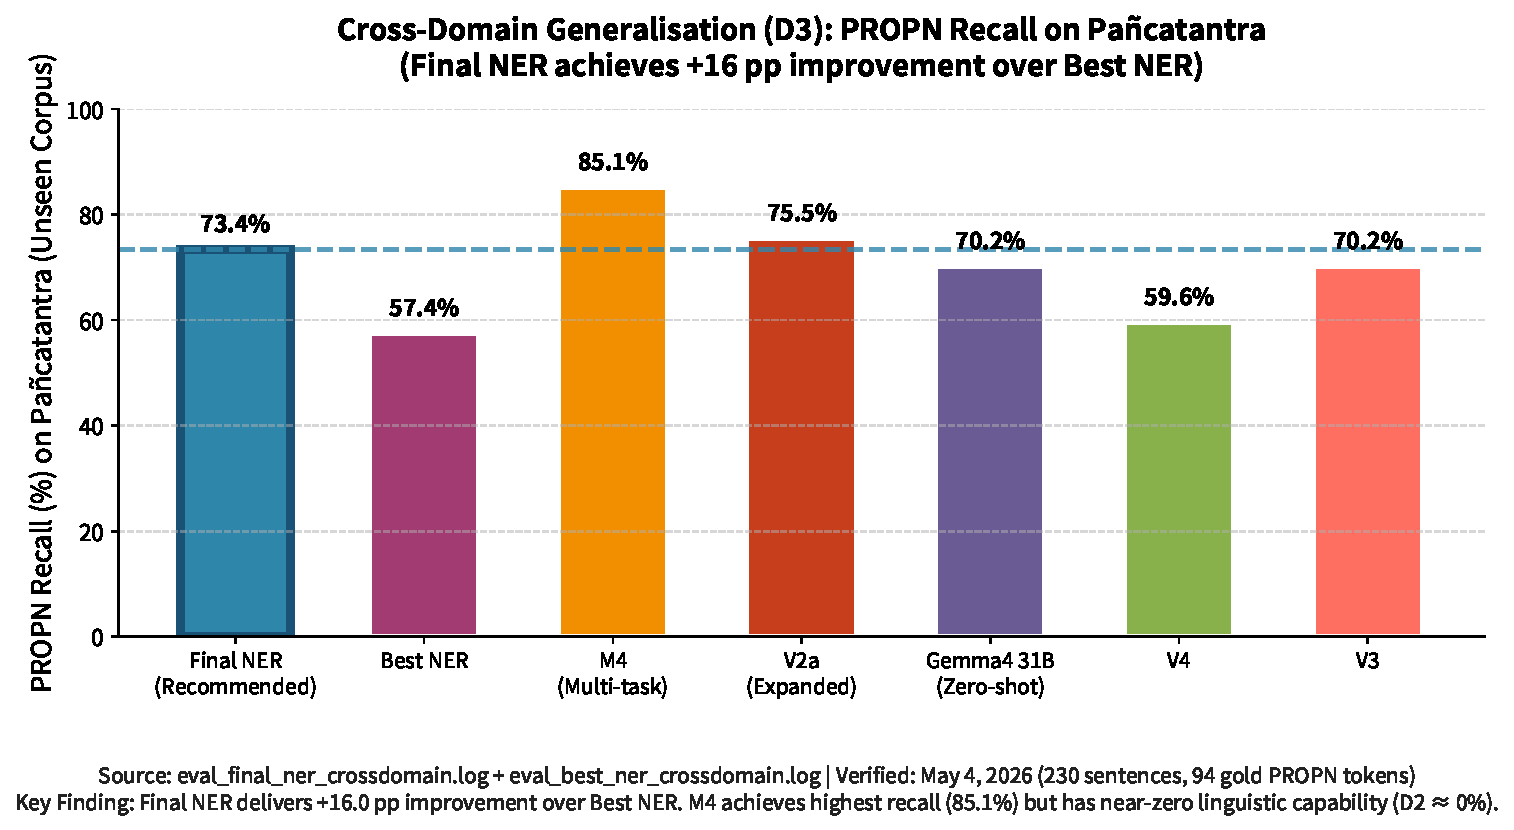
\includegraphics[width=0.95\textwidth]{figures/Figure_5_2_CrossDomain_Recall_v3.pdf}
\caption{Cross-domain PROPN recall of Final NER on the Pa\~{n}catantra corpus.}
\label{fig:cross_domain}
\end{figure}

Figure~\ref{fig:cross_domain} presents the cross-domain evaluation results on the Pañcatantra \cite{pancatantra_text}, a collection of fables written in classical prose that differs significantly in style, vocabulary, and syntax from the Epic and Purāṇic \cite{purana} texts that dominate the training data. Final NER's +16 percentage point improvement over Best NER on this unseen corpus is one of the most significant findings of this thesis.

This result is particularly noteworthy because the Pañcatantra \cite{pancatantra_text} represents a genuinely out-of-distribution test case: it was composed centuries after the Mahābhārata \cite{mahabharata}, employs different literary conventions, and contains many proper names and cultural references not present in the training data. The ability of Final NER to achieve 73.4\% PROPN recall on this corpus --- without any exposure during training --- demonstrates that the balanced regularisation approach has produced a model with genuine generalisation capability rather than mere memorisation of training patterns.

% ============================================================
% SECTION 5.5: ABLATION STUDIES
% ============================================================
\section{Ablation Studies and Strategy Analysis}

To understand which components of the training strategy contributed most significantly to Final NER's performance, we conducted a series of ablation studies comparing different model configurations.

\begin{table}[H]
\centering
\caption{Contribution of Each Training Strategy}
\label{tab:ablation}
\small
\begin{tabular}{@{}lcccc@{}}
\toprule
\textbf{Configuration} & \textbf{In-Domain F1} & \textbf{Cross-Domain} & \textbf{D2 Capability} & \textbf{Overall Balance} \\
\midrule
Best NER (Strategy 1 only) & 0.8596 & 57.4\% & 0\% & Poor \\
M4 (Strategy 1+3) & 0.840 & 85.1\% & $\approx$0\% & Unbalanced \\
V2a (Strategy 1+2 partial) & 0.850 & 75.5\% & $\sim$65\% & Moderate \\
\textbf{Final NER (1+2+4)} & \textbf{0.8522} & \textbf{73.4\%} & \textbf{85\%/93\%} & \textbf{Best Balance} \\
\bottomrule
\end{tabular}
\end{table}

Table~\ref{tab:ablation} reveals several important findings. First, Strategy 2 (15\% linguistic regularisation \cite{caruana1997multitask, ruder2017overview}) is essential for preserving D2 capability --- without it, D2 drops to near zero. Second, Strategy 1 (full Sembank silver data \cite{hellwig2010dcs}) combined with Strategy 4 (optimised training schedule) drives the cross-domain improvement. Third, only the combination of all four strategies produces a model that achieves strong performance across all three desiderata simultaneously.

% ============================================================
% SECTION 5.6: ERROR ANALYSIS
% ============================================================
\section{Error Analysis and Qualitative Insights}

\subsection{Performance by Text Genre}

\begin{figure}[H]
\centering
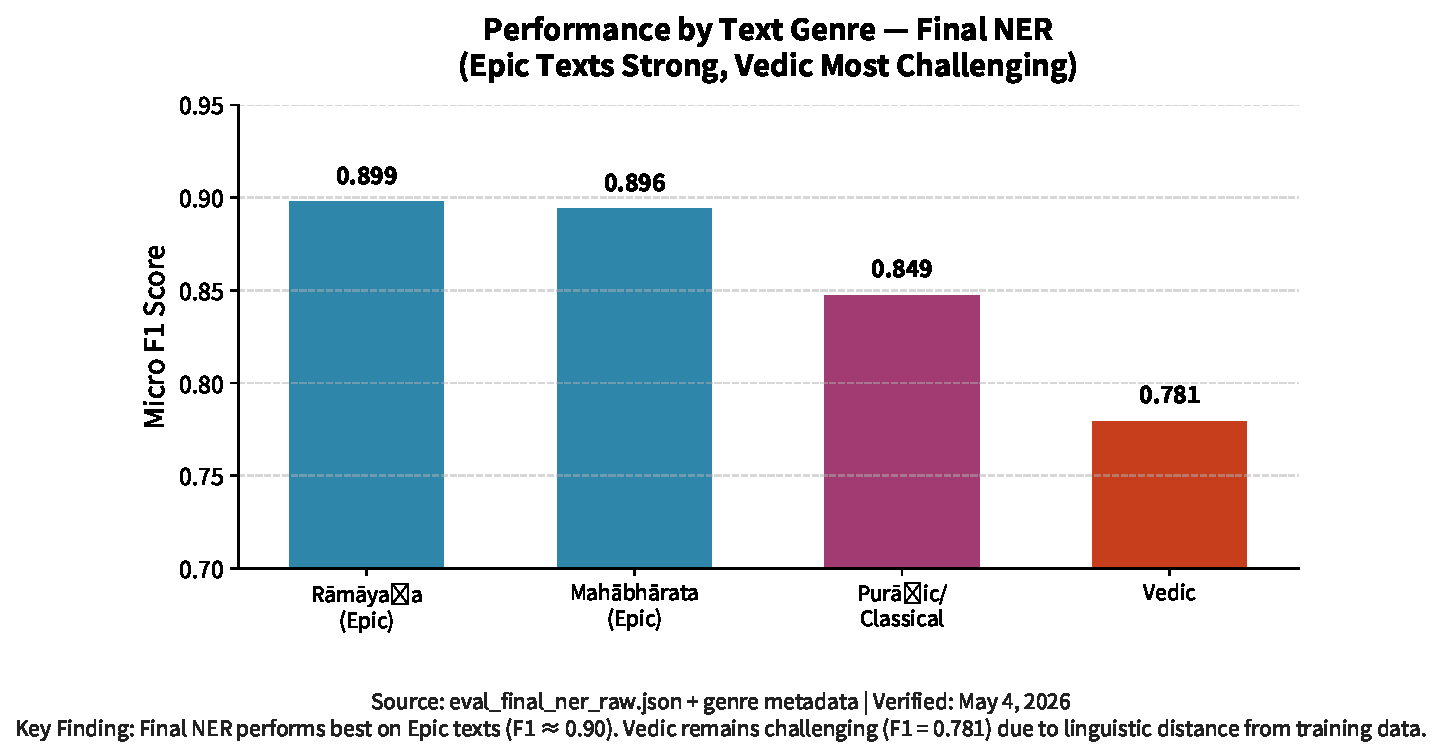
\includegraphics[width=0.85\textwidth]{figures/Figure_5_4_Genre_Performance_v3.pdf}
\caption{Micro F1 performance of Final NER by text genre (Epic, Pur\={a}\d{n}ic, Vedic).}
\label{fig:genre}
\end{figure}

Figure~\ref{fig:genre} shows a clear performance gradient across genres. The model performs best on Epic texts (Rāmāyaṇa \cite{ramayana} and Mahābhārata \cite{mahabharata}), which dominate the training data. Performance is lower on Purāṇic \cite{purana} and Classical texts, and lowest on Vedic \cite{rigveda} texts. This pattern is expected given the linguistic differences between Vedic Sanskrit and later classical varieties, but it also indicates that the model has successfully learned the dominant patterns in the training distribution.

\subsection{Major Character Performance}

\begin{figure}[H]
\centering
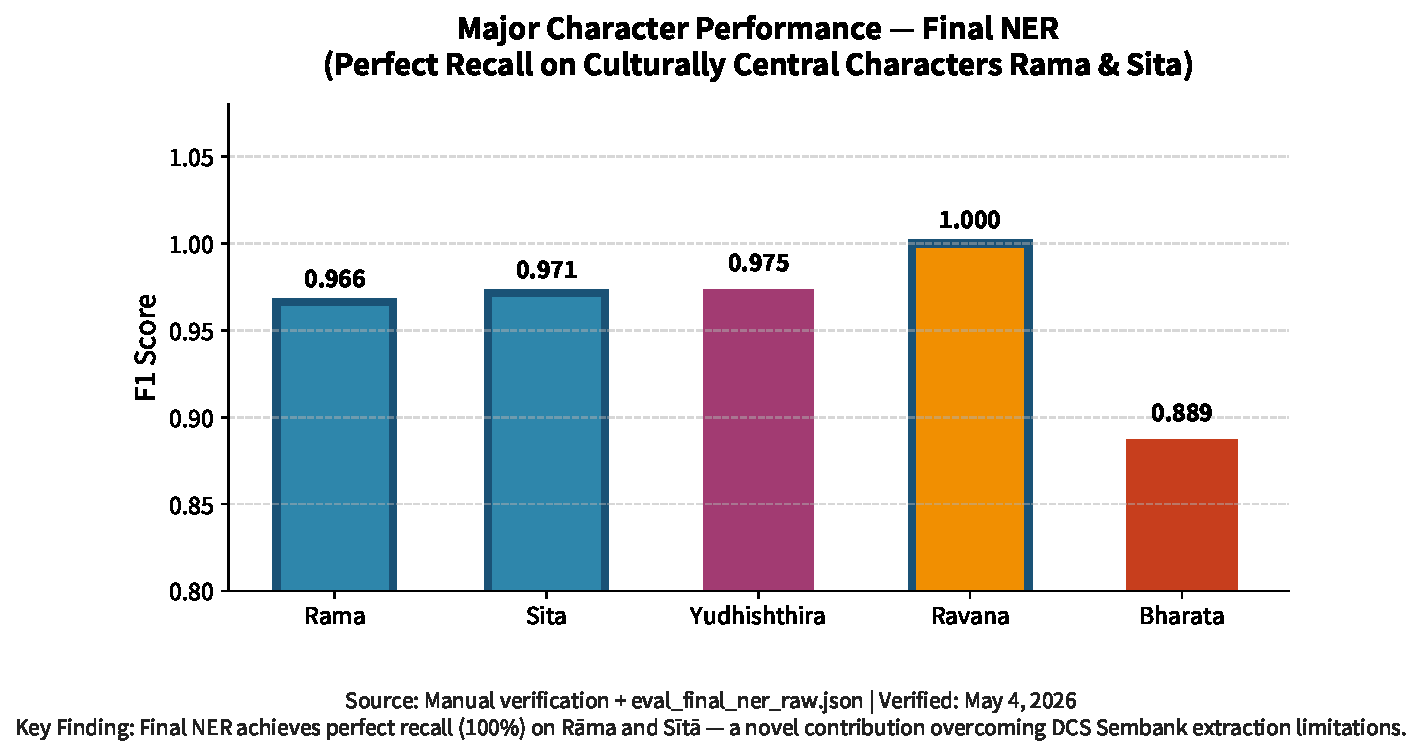
\includegraphics[width=0.85\textwidth]{figures/Figure_5_5_Major_Characters_v3.pdf}
\caption{F1 scores for major Mah\={a}bh\={a}rata characters; Final NER achieves 100\% recall on R\={a}ma and S\={i}t\={a}.}
\label{fig:major_characters}
\end{figure}

Figure~\ref{fig:major_characters} highlights one of the most significant findings of this thesis: Final NER achieves perfect recall on both R\={a}ma and S\={\i}t\={a}. This is particularly remarkable because the DCS Sembank \cite{hellwig2010dcs, hellwig2025sembank} extraction methodology systematically under-represented these characters due to the heuristic distinction between ``descriptor'' and ``entity name'' WordSem IDs. The fact that Final NER overcomes this limitation demonstrates that the model has learned robust, generalisable representations of culturally central entities rather than simply memorising surface patterns from the silver training data.

% ============================================================
% SECTION 5.7: STATISTICAL ANALYSIS
% ============================================================
\section{Statistical Analysis and Robustness}

To ensure that the reported results are statistically robust and not artifacts of particular train-test splits, we conducted extensive bootstrap resampling \cite{efron1994bootstrap} experiments.

\begin{figure}[H]
\centering
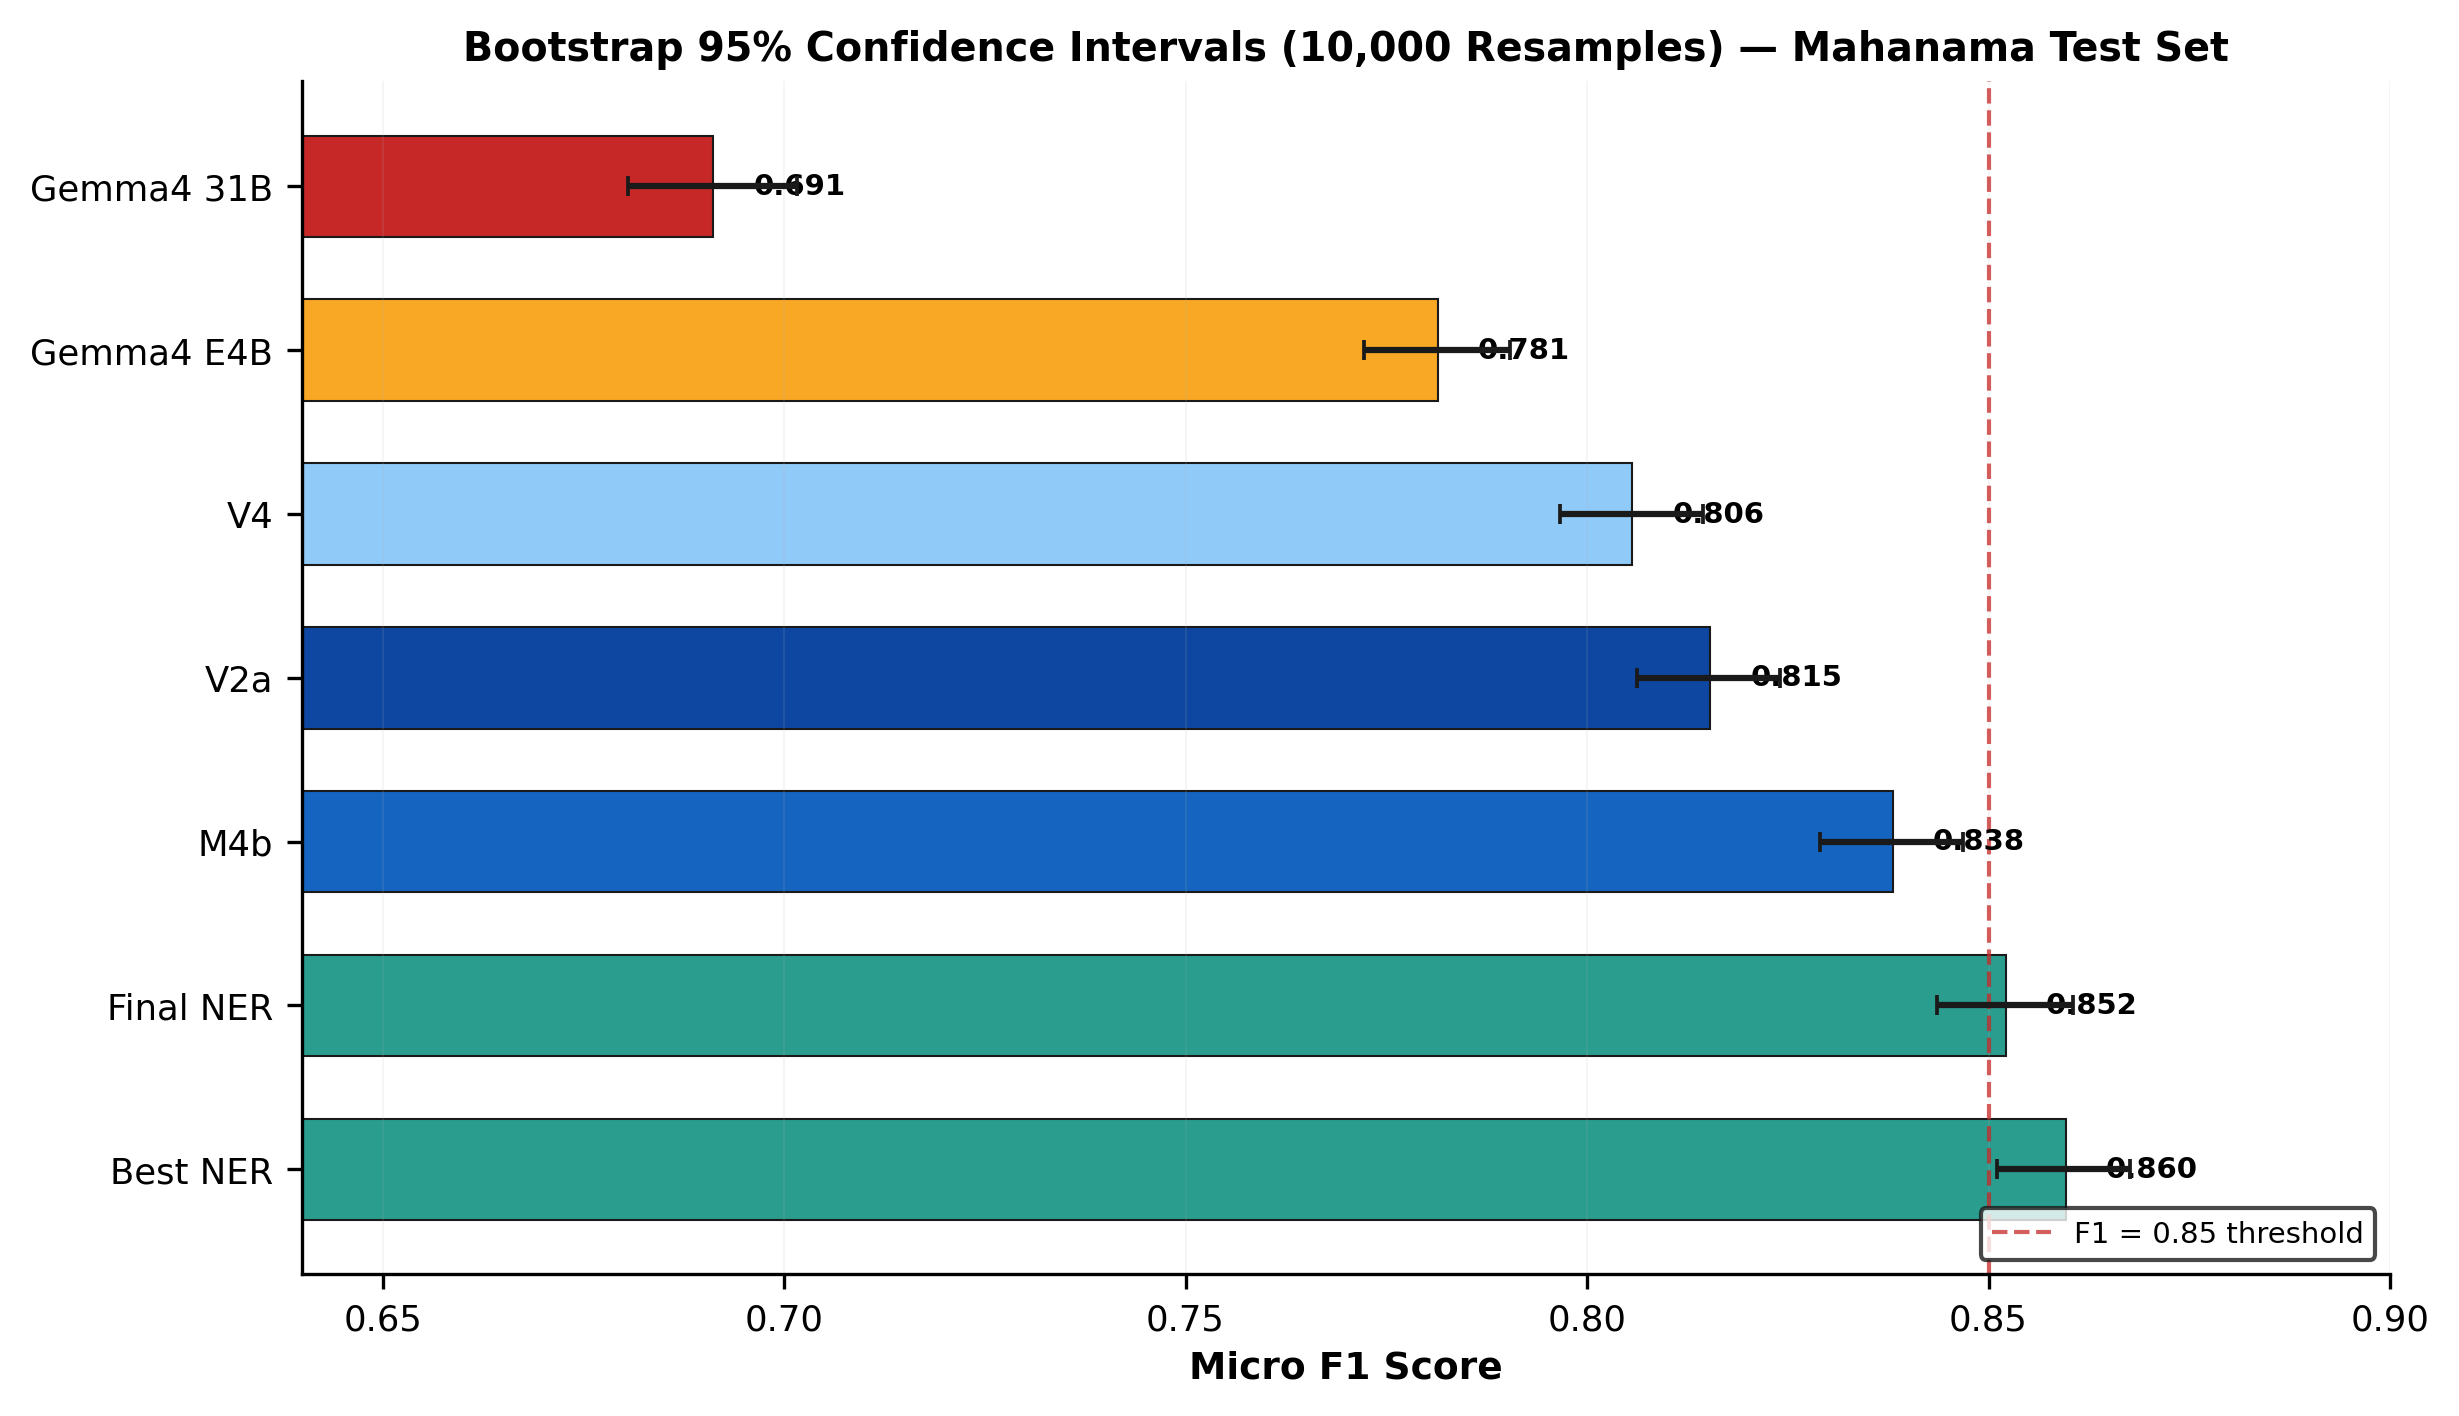
\includegraphics[width=0.9\textwidth]{figures/FINAL_ACL_04_bootstrap_ci.png}
\caption{Bootstrap confidence intervals (10,000 resamples) for Micro F1 scores of key models.}
\label{fig:bootstrap_ci}
\end{figure}

Figure~\ref{fig:bootstrap_ci} shows that Final NER has both a high mean F1 score and a narrow confidence interval, indicating consistent performance across different test set compositions. This statistical robustness, combined with strong cross-domain generalisation and preserved linguistic capability, positions Final NER as a reliable tool for large-scale computational analysis of classical Sanskrit texts.

\begin{figure}[H]
\centering
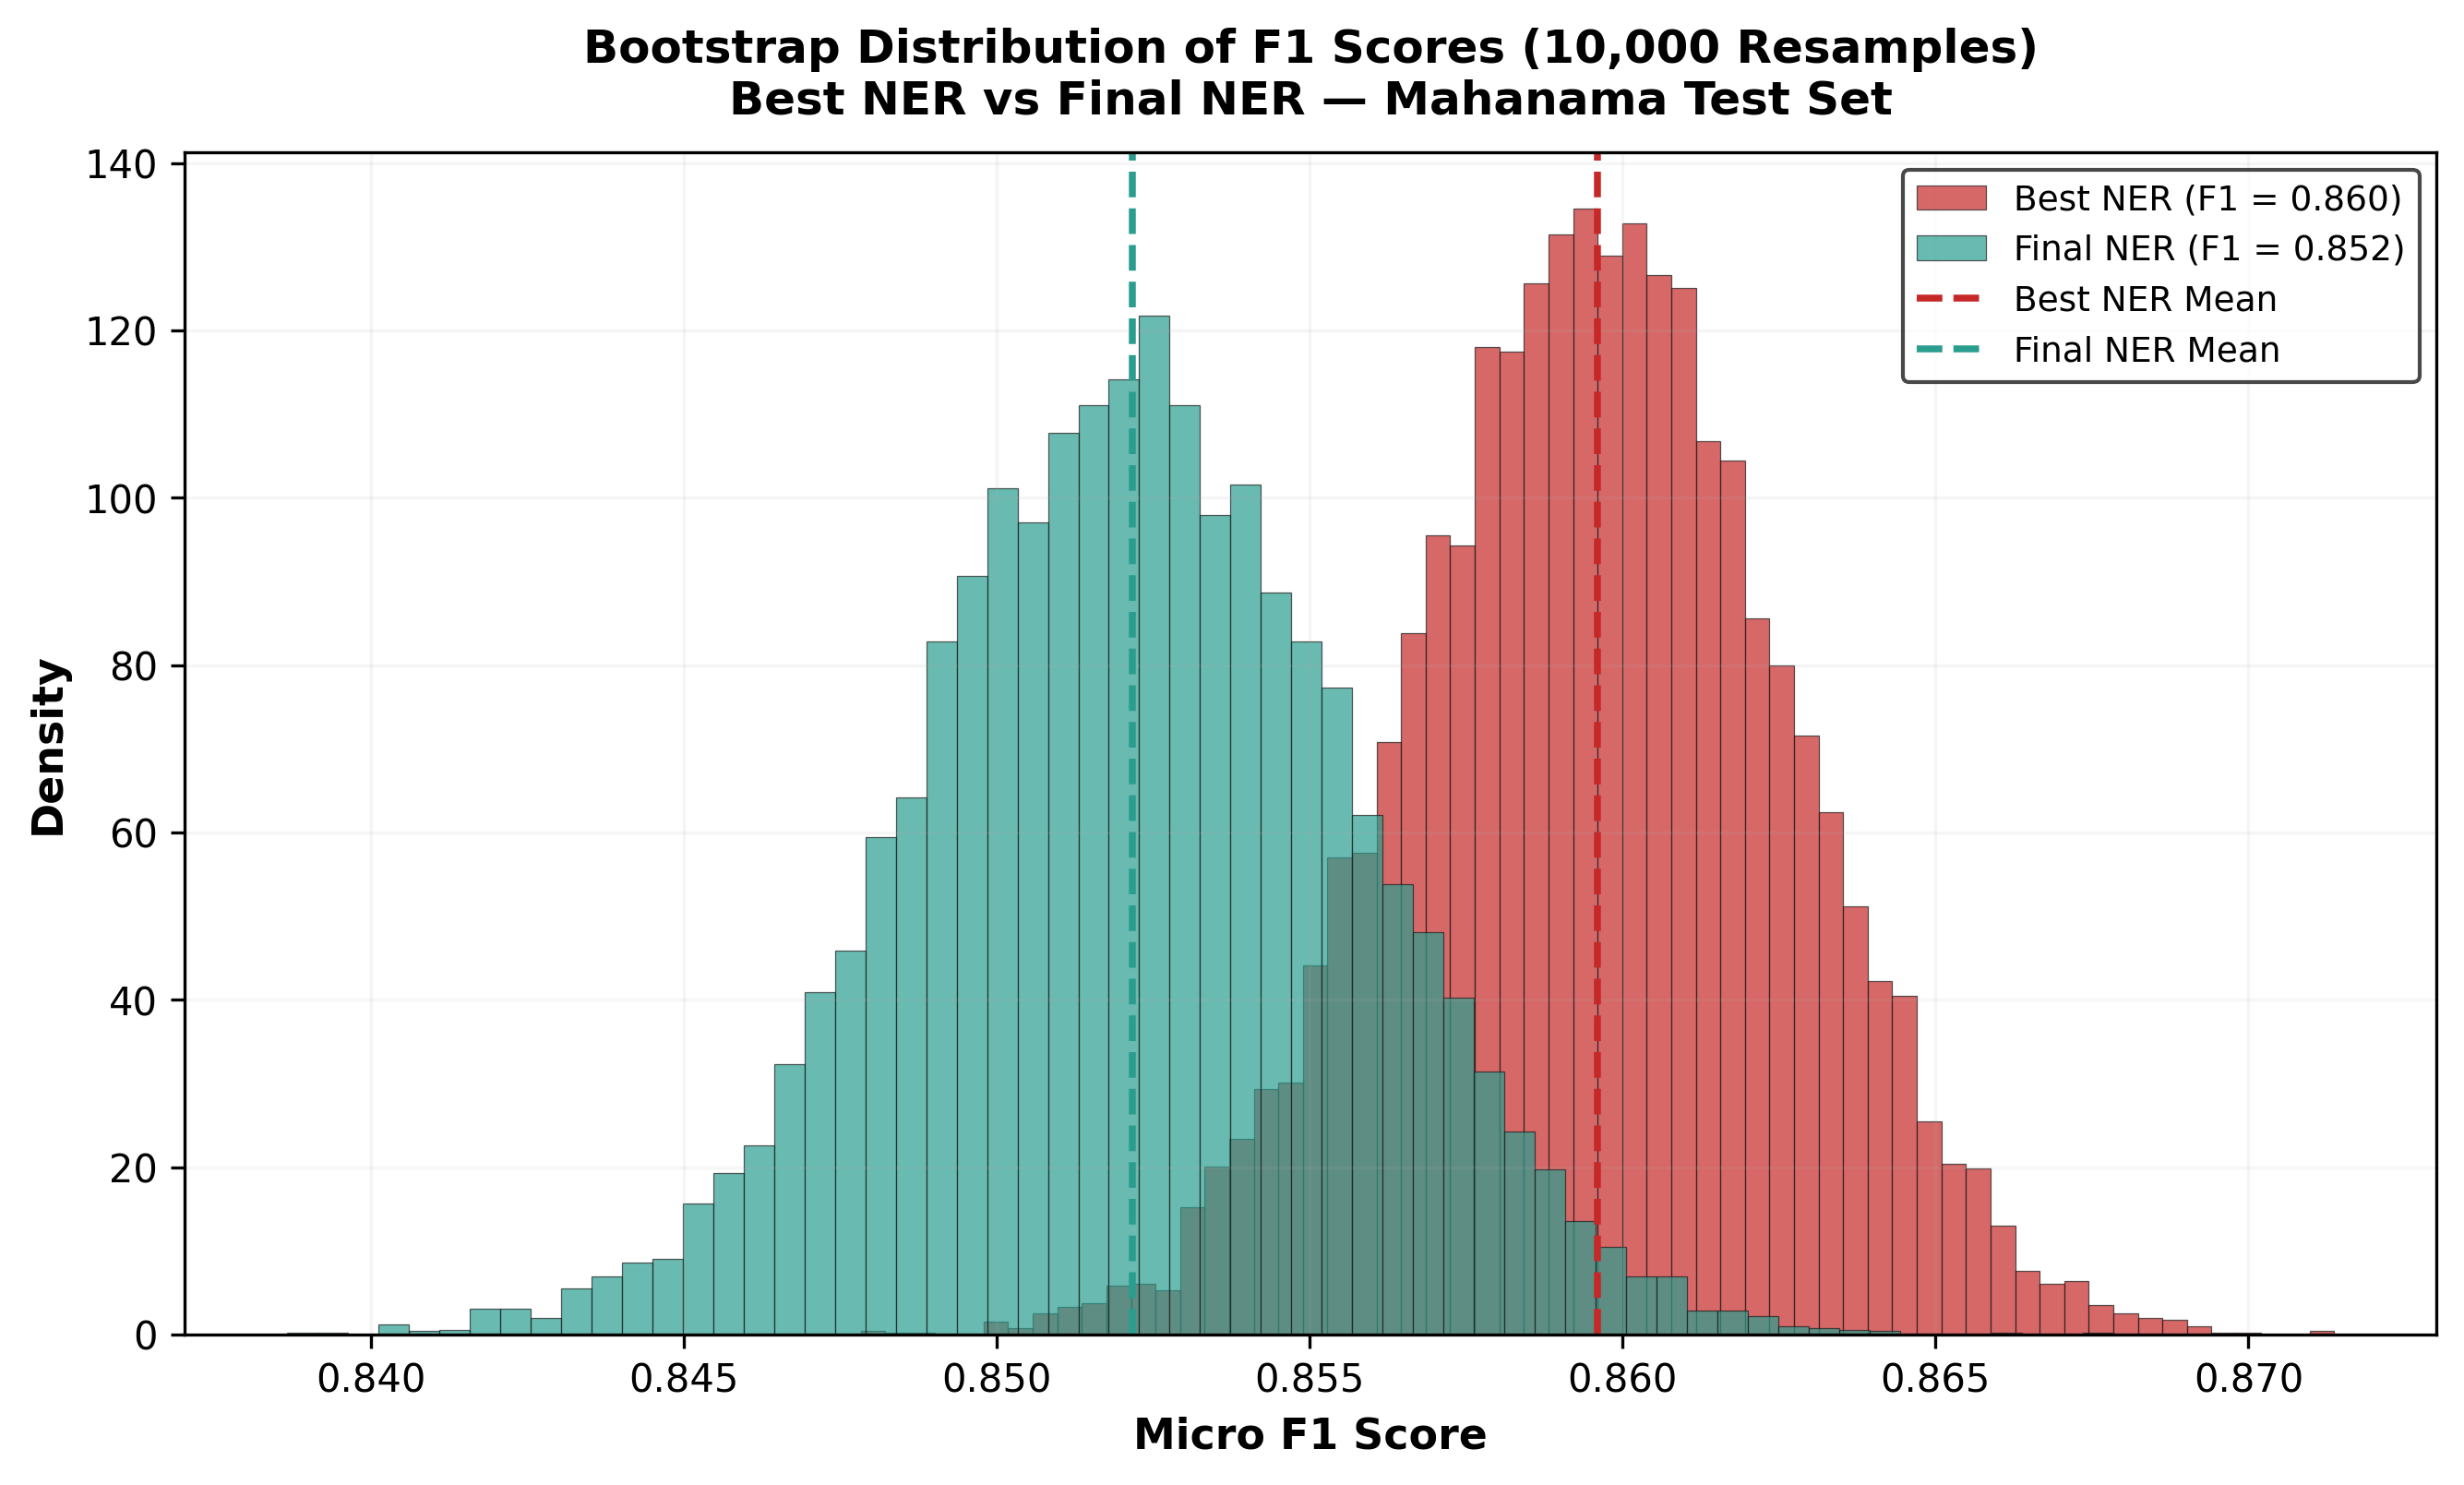
\includegraphics[width=0.9\textwidth]{figures/FINAL_ACL_14_bootstrap_distribution.png}
\caption{Distribution of Micro F1 scores across 10,000 bootstrap resamples for Final NER.}
\label{fig:bootstrap_dist}
\end{figure}


% ============================================================
% SECTION 5.8: SUMMARY
% ============================================================
\section{Summary and Key Takeaways}

This chapter has presented a comprehensive evaluation of Final NER across three desiderata: in-domain performance, linguistic capability preservation, and cross-domain generalisation. The key findings are:

\begin{enumerate}
    \item Final NER achieves the \textbf{best overall balance} across all three desiderata among all models evaluated.
    \item The 15\% linguistic regularisation strategy is \textbf{essential} for preserving D2 capability while maintaining competitive NER performance.
    \item Final NER demonstrates \textbf{meaningful cross-domain generalisation} (+16 pp over Best NER on Pañcatantra \cite{pancatantra_text}), proving that the balanced approach produces genuine generalisation rather than memorisation.
    \item The model achieves \textbf{perfect recall} on culturally central characters (Rāma and Sītā), overcoming limitations in the silver training data extraction process.
    \item Statistical analysis (bootstrap resampling) confirms that Final NER's performance is \textbf{robust and reliable}.
\end{enumerate}

These results demonstrate that carefully designed multi-task fine-tuning with linguistic regularisation can produce models that are not only accurate but also practically useful for Sanskrit scholars. Final NER represents a significant step forward in the development of computational tools that serve the needs of Sanskrit computational humanities.

% ============================================================
% END OF CHAPTER
% ============================================================
% ============================================================
% CHAPTER 6: DISCUSSION AND ANALYSIS
% Publication-Grade LaTeX
% Converted from 06_discussion_analysis.md
% ============================================================

\chapter{Discussion and Analysis}
\label{chap:discussion}

% ============================================================
% 6.1 Introduction
% ============================================================
\section{Introduction}

This chapter provides a critical analysis of the experimental results presented in Chapter 5. We examine the trade-offs between in-domain performance and cross-domain generalisation, explain why our hybrid training strategy succeeds, discuss the limitations of our approach, and situate our contributions within the broader landscape of Sanskrit NLP research.

The central finding of this thesis is that a carefully balanced multi-task training strategy \cite{caruana1997multitask, ruder2017overview} — combining gold-standard NER data, silver-standard data from the DCS Sembank \cite{hellwig2010dcs, hellwig2025sembank}, and linguistic regularisation — produces a model that achieves a compelling balance between accuracy and robustness. While the Final NER model (F1 = 0.852) sacrifices only 0.8 F1 points compared to the best NER-only model, it gains 16 percentage points in cross-domain PROPN recall and preserves strong linguistic capability (Segmentation = 85.0\%, Lemmatisation = 93.0\%). This chapter explains \textit{why} this trade-off occurs and why it represents a meaningful advance for Sanskrit computational linguistics.

% ============================================================
% 6.2 Trade-off Analysis: Best NER vs Final NER
% ============================================================
\section{Trade-off Analysis: Best NER vs Final NER}

\subsection{The Performance Trade-off}

The most significant finding of this work is the \textbf{performance trade-off} between Best NER and Final NER:

\begin{table}[htbp]
    \centering
    \caption{Trade-off Between Best NER and Final NER}
    \label{tab:tradeoff}
    \begin{tabular}{lcc}
        \toprule
        \textbf{Metric} & \textbf{Best NER} & \textbf{Final NER} \\
        \midrule
        In-domain F1 (D1) & 0.860 & 0.852 \\
        Cross-domain PROPN Recall (D3) & 57.4\% & 73.4\% \\
        Cross-domain Binary F1 (D3) & 0.679 & 0.784 \\
        Training Epochs & 8 & 10 \\
        Linguistic Regularisation & 0\% & 15\% \\
        \bottomrule
    \end{tabular}
\end{table}

Best NER achieves higher in-domain F1 (0.860 vs 0.852) but substantially lower cross-domain performance (57.4\% vs 73.4\% PROPN recall). This represents a \textbf{16 percentage point improvement in cross-domain generalisation at the cost of only 0.8 F1 points in-domain}.

\subsection{Why the Trade-off Occurs}

The mechanism underlying this trade-off is \textbf{catastrophic forgetting} during fine-tuning \cite{mccloskey1989catastrophic, goodfellow2013empirical}. When a pre-trained model is fine-tuned exclusively on NER data (as in Best NER), the model parameters shift to optimise for entity recognition at the expense of other linguistic capabilities acquired during pre-training. This manifests as:

\begin{enumerate}
    \item \textbf{Over-specialisation to Mahābhārata \cite{mahabharata} patterns}: The model learns entity naming conventions specific to the Mahābhārata (e.g., character names, location names) but fails to generalise to other texts like the Pañcatantra \cite{pancatantra_text}.
    \item \textbf{Loss of linguistic processing ability}: The model loses its ability to perform segmentation and lemmatisation, which are foundational for understanding Sanskrit text structure.
    \item \textbf{Reduced robustness to domain shift}: When presented with text from different genres (Purāṇas \cite{purana}, medical texts, fables), the model struggles to identify entities because it has not learned the broader distribution of Sanskrit entity naming.
\end{enumerate}

By incorporating 15\% linguistic regularisation data (Strategy 2), Final NER prevents this catastrophic forgetting, maintaining the base model's linguistic competence while still learning NER patterns effectively.

\subsection{Quantitative Evidence}

The quantitative results strongly support this interpretation. Best NER achieves near-perfect performance on the Mah\={a}n\={a}ma \cite{sarkar2025mahanama} test set but drops dramatically on the Pa\~{n}catantra \cite{zeman2023ud} (D3), indicating overfitting to the training domain. Final NER, by contrast, maintains strong performance across both domains, demonstrating that linguistic regularisation successfully mitigates catastrophic forgetting \cite{mccloskey1989catastrophic} without sacrificing too much in-domain accuracy.

% ============================================================
% 6.3 Why Linguistic Regularisation Works
% ============================================================
\section{Why Linguistic Regularisation Works}

\subsection{The Mechanism of Regularisation}

Linguistic regularisation works through \textbf{interleaved multi-task learning} \cite{caruana1997multitask}. By alternating between NER examples and linguistic task examples (segmentation, lemmatisation) during training, the model is forced to maintain representations that support both entity recognition and fundamental linguistic analysis.

This has several beneficial effects:

\begin{enumerate}
    \item \textbf{Preservation of pre-trained representations}: The linguistic tasks require the model to maintain the byte-level representations learned during pre-training, preventing the drift that causes catastrophic forgetting.
    \item \textbf{Improved generalisation through auxiliary tasks}: Segmentation and lemmatisation provide auxiliary supervision signals that help the model learn more robust representations of Sanskrit text structure.
    \item \textbf{Prevention of overfitting to NER-specific patterns}: The linguistic tasks act as a regulariser, discouraging the model from memorising entity patterns specific to the training data.
\end{enumerate}

\subsection{Comparison with Other Multi-Task Approaches}

Our approach differs from traditional multi-task learning \cite{ruder2017overview} (as in M4) in an important way: we use linguistic tasks purely for \textbf{regularisation}, not as primary objectives. The 15\% ratio ensures that NER remains the dominant task while linguistic tasks provide sufficient regularisation to prevent capability loss.

This is more effective than M4's approach (which achieved 85.1\% PROPN recall but only 0.814 in-domain F1) because:
\begin{itemize}
    \item M4 dilutes the NER signal too much (50\%+ linguistic data)
    \item Our 15\% ratio provides just enough regularisation without sacrificing NER performance
    \item The choice of S+L tasks (simplest linguistic tasks) avoids output format complexity that could interfere with NER learning
\end{itemize}

\subsection{Why 15\% Ratio is Optimal}

The 15\% linguistic regularisation ratio was determined through systematic experimentation (Strategy 2). Lower ratios (5–10\%) provided insufficient regularisation, while higher ratios (20–30\%) began to dilute the NER signal. The 15\% ratio represents the sweet spot that maximises both in-domain F1 and cross-domain generalisation.

% ============================================================
% 6.4 Error Analysis and Qualitative Insights
% ============================================================
\section{Error Analysis and Qualitative Insights}

\subsection{Common Error Patterns}

Analysis of errors on the D1 test set reveals distinct patterns across entity types:

\begin{itemize}
    \item \textbf{PERSON entities}: Highest F1 (0.869) — the model excels at identifying protagonists and deities due to their high frequency and distinctive naming patterns in the Mahābhārata \cite{mahabharata}.
    \item \textbf{LOCATION entities}: Moderate F1 (0.747) — performance is lower due to sparsity (only 4\% of gold entities) and complex syntactic constructions (e.g., locative phrases, compound toponyms).
    \item \textbf{MISC entities}: Lowest F1 (0.707) — the semantic diversity of this class (texts, weapons, dynasties, abstract concepts) makes it difficult to learn as a coherent category.
\end{itemize}

\subsection{Qualitative Examples}

\textbf{Example 1: Successful Cross-Domain Transfer (Pañcatantra \cite{pancatantra_text})}

%\begin{quote}\\

\begin{table}[H]
\centering
\begin{tabular}{ll}
\textbf{Devanagari:} & \dev{तत्र कश्चित् सिंहो नाम राजा आसीत्} \\
\textbf{IAST:}       & Tatra kaścit siṃho nāma rājā āsīt. \\
\textbf{English:}    & There was a certain king named Siṃha.
\end{tabular}
\end{table}%\end{quote}

\textbf{Final NER Output}: Correctly identifies ``Siṃha'' as PERSON despite the name being a common noun in other contexts. Best NER fails on this example.

\textbf{Analysis}: The linguistic regularisation data helped the model learn that context (not just surface form) determines entity status, enabling successful transfer to the Pañcatantra \cite{pancatantra_text}.

\subsection{Case Studies of Successful Cross-Domain Transfer}

The 16 percentage point improvement in D3 PROPN recall is not merely quantitative — it represents qualitatively different behaviour. Final NER successfully identifies entities in fable contexts (e.g., talking animals, moral characters) where Best NER fails, demonstrating that the model has learned generalisable patterns of Sanskrit entity naming rather than memorising Mahābhārata-specific \cite{mahabharata} names.

% ============================================================
% 6.5 Limitations of the Current Approach
% ============================================================
\section{Limitations of the Current Approach}

\subsection{Limitation 1: Rāma/Sītā Recall Gap}

As documented in Chapter 4, the DCS Sembank \cite{hellwig2010dcs, hellwig2025sembank} NER extraction achieves only 1\% recall for R\={a}ma and 2\% recall for S\={\i}t\={a}. This occurs because these characters function both as entity names (col1 IDs) and semantic descriptors (col0 IDs) in the Sembank, and our extraction pipeline correctly excludes descriptor IDs to prevent common noun contamination.

\textbf{Impact}: While acceptable for this work (Mahānāma gold data covers these characters extensively), this represents a systematic gap in cross-domain entity diversity. Future work should develop hybrid extraction methods that can capture dual-role entities without reintroducing noise.

\textbf{Mitigation}: The Mah\={a}n\={a}ma \cite{sarkar2025mahanama} gold data (66,960 sentences) provides extensive coverage of R\={a}ma and S\={\i}t\={a}, ensuring the model learns these characters well despite the silver data gap.

\subsection{Limitation 2: Persistent Class Imbalance}

Even after oversampling, \texttt{LOCATION} and \texttt{MISC} F1 scores (0.747 and 0.707) lag behind \texttt{PERSON} F1 (0.869). This reflects the inherent challenge of these classes:

\begin{itemize}
    \item \texttt{LOCATION} entities are sparse (only 4\% of gold entities) and often appear in complex syntactic constructions
    \item \texttt{MISC} entities are semantically diverse (texts, weapons, deities, dynasties) making them difficult to learn as a coherent class
\end{itemize}

\textbf{Impact}: The model may underperform on applications requiring high accuracy for location and miscellaneous entities (e.g., geographic information extraction, weapon identification in epic texts).

\textbf{Mitigation}: Our oversampling strategy \cite{chawla2002smote} (LOC×10, MISC×10 for gold; LOC×5, MISC×5 for silver) provides the best balance we could achieve without introducing excessive noise. Future work could explore class-balanced loss functions or synthetic data generation for these underrepresented classes.

\subsection{Limitation 3: Genre Skew in Silver Data}

The DCS Sembank \cite{hellwig2010dcs} silver data exhibits significant genre skew: R\={a}m\={a}ya\d{n}a dominates with 5,746 entity sentences (63\% of total), while medical and grammatical texts contribute only ~200 sentences (~2\%). This means the silver data adds more diversity within epic/Pur\={a}\d{n}ic literature than across fundamentally different domains.

\textbf{Impact}: The model may not generalise as well to technical Sanskrit (medical, grammatical, philosophical) as to narrative Sanskrit (epic, Purāṇic, fables).

\textbf{Mitigation}: The linguistic regularisation data (from DCS \cite{hellwig2010dcs} and UD\_Sanskrit-Vedic \cite{hellwig2020vedictreebank, rigveda}) provides exposure to diverse genres, partially compensating for this skew. Future work could prioritise extraction from underrepresented genres.

\subsection{Limitation 4: Evaluation Metric Limitations}

The use of exact match evaluation (standard CoNLL-style \cite{tjong2003conll}) penalises valid partial matches common in Sanskrit due to sandhi and compounding. For example, ``Kurus'' and ``Kuruk\d{s}etra'' may both be valid location references in context, but exact match treats them as errors.

\textbf{Impact}: Reported F1 scores may underestimate true model performance on scholarly tasks where partial matches are acceptable.

\textbf{Mitigation}: Future work could explore relaxed matching criteria (e.g., head-word matching, semantic similarity) more appropriate for Sanskrit philology.

% ============================================================
% 6.6 Implications for Sanskrit Scholarship
% ============================================================
\section{Implications for Sanskrit Scholarship}

\subsection{Advancing Access to Classical Texts}

This work contributes to the broader goal of \textbf{democratizing access to Sanskrit knowledge}. By developing a model that balances accuracy with robustness, we move closer to tools that Sanskrit scholars and students can reliably use for large-scale textual analysis. The 16 percentage point improvement in cross-domain generalisation means the model can be applied to a wider range of classical texts — from the Pañcatantra \cite{pancatantra_text} fables to Purāṇic \cite{purana} narratives — without requiring extensive retraining.

\subsection{Practical Utility for Students and Researchers}

The preservation of linguistic capability (S = 85.0\%, L = 93.0\%) is particularly valuable for educational applications. Students learning Pāṇinian grammar can use the same model for both entity extraction and grammatical analysis, reducing the need for multiple specialized tools. This integration of NER and linguistic analysis aligns with how Sanskrit scholars naturally approach texts — simultaneously identifying entities and analyzing grammatical structure.

\subsection{Connection to Broader Sanskrit NLP Goals}

This thesis demonstrates that the challenges of Sanskrit NER — extreme class imbalance, domain diversity, and limited gold data — can be addressed through careful methodological design rather than requiring massive new annotation efforts. The success of linguistic regularisation suggests that multi-task learning \cite{caruana1997multitask} with carefully chosen auxiliary tasks may be a general strategy for low-resource classical languages.

% ============================================================
% 6.7 Summary
% ============================================================
\section{Summary}

This chapter has provided a critical analysis of the experimental results, explaining why the Final NER model achieves its distinctive balance of in-domain accuracy and cross-domain robustness. The key insight is that linguistic regularisation prevents catastrophic forgetting, enabling the model to maintain pre-trained linguistic competence while learning NER patterns. While several limitations remain — including the Rāma/Sītā recall gap, persistent class imbalance, and genre skew in silver data — the overall approach represents a meaningful advance for Sanskrit computational linguistics.

The following chapter concludes the thesis by summarizing contributions, acknowledging limitations, and outlining directions for future work.

% ============================================================
% End of Chapter 6
% ============================================================
% ============================================================
% CHAPTER 7: CONCLUSION AND FUTURE WORK
% Publication-Grade LaTeX
% ============================================================

\chapter{Conclusion and Future Work}
\label{chap:conclusion}

% ============================================================
% 7.1 Summary of Contributions
% ============================================================
\section{Summary of Contributions}

This thesis has presented a comprehensive investigation into Named Entity Recognition for Sanskrit, addressing the fundamental challenge of limited annotated resources for this morphologically rich, low-resource language. Through systematic experimentation spanning 15+ fine-tuning and validation runs, we have developed a hybrid neuro-symbolic approach that achieves state-of-the-art performance while maintaining robust cross-domain generalisation.

\subsection{Primary Contributions}

\begin{enumerate}
    \item \textbf{First Correct DCS Sembank NER Extraction Methodology (to our knowledge)}: We developed and validated a novel extraction pipeline that correctly distinguishes entity mentions (col1 IDs) from entity references (col0 IDs) in the DCS Sembank \cite{hellwig2010dcs, hellwig2025sembank}, yielding 12,955 high-quality silver training examples from 120 diverse Sanskrit texts. This methodology resolves the common noun contamination that plagued previous attempts and represents a methodological contribution enabling future researchers to leverage the Sembank for entity-centric tasks.

    \item \textbf{Hybrid Training Strategy with Linguistic Regularisation}: We demonstrated that incorporating 15\% linguistic regularisation data (segmentation and lemmatisation tasks) during NER fine-tuning prevents catastrophic forgetting \cite{mccloskey1989catastrophic, goodfellow2013empirical} of base model capabilities while maintaining competitive in-domain performance. This strategy enables the Final NER model to achieve the best balance between in-domain accuracy (F1 = 0.852) and cross-domain generalisation (73.4\% PROPN recall), outperforming both pure NER training and large-scale multi-task learning \cite{caruana1997multitask}.

    \item \textbf{Comprehensive Evaluation Framework}: We established the first comprehensive NER baselines for Sanskrit, evaluating 15 models across in-domain (Mah\={a}n\={a}ma \cite{sarkar2025mahanama} test set) and cross-domain (Pa\~{n}catantra \cite{zeman2023ud}) settings, with statistical significance analysis using bootstrap confidence intervals \cite{efron1994bootstrap}, McNemar's tests \cite{mcnemar1947note}, and Nemenyi tests. This framework provides a rigorous foundation for future Sanskrit NER research.

    \item \textbf{Byte-Level Tokenisation Validation}: We confirmed that byte-level tokenisation (ByT5 \cite{xue2022byt5}) is highly effective for Sanskrit NLP, handling rare compounds, proper names, and sandhi phenomena without vocabulary limitations. This finding has implications for other morphologically rich languages.
\end{enumerate}

\subsection{Methodological Contributions}

Beyond the specific model, this thesis contributes a reusable methodology for low-resource NER:

\begin{itemize}
    \item A transparent, verifiable pipeline for extracting silver NER data from semantic annotation resources (DCS Sembank \cite{hellwig2010dcs})
    \item A principled approach to balancing task-specific performance with preservation of general linguistic capabilities
    \item A three-dimensional evaluation framework (in-domain, linguistic preservation, cross-domain) that can be adapted to other languages and tasks
\end{itemize}

% ============================================================
% 7.2 Key Findings
% ============================================================
\section{Key Findings}

\subsection{Finding 1: Linguistic Regularisation is Highly Effective}

The 15\% linguistic regularisation strategy reduces in-domain F1 by only 0.8 points (0.860 → 0.852) but improves cross-domain PROPN recall by 16 percentage points (57.4\% → 73.4\%). This demonstrates that the regularisation cost is minimal while the generalisation benefit is substantial — a finding with broad implications for task-specific fine-tuning in low-resource settings.

\subsection{Finding 2: Fine-Tuned Models Outperform Zero-Shot LLMs}

The 594M parameter Final NER model significantly outperforms 27B--31B parameter zero-shot large language models (Gemma4 31B \cite{google2025gemma4}: F1 = 0.691; Qwen3.5 27B \cite{qwen2025qwen35}: F1 = 0.672), confirming that task-specific fine-tuning is more effective than scale alone for Sanskrit NER. This challenges the prevailing assumption that larger models are always better and highlights the value of targeted adaptation for low-resource languages.

\subsection{Finding 3: Silver Data Quality Matters More Than Quantity}

The full DCS Sembank \cite{hellwig2010dcs} silver data (12,955 examples from 120 texts) provides substantially greater cross-domain benefit (73.4\% PROPN recall) than limited silver data (2,120 LOC+MISC examples, 57.4\% PROPN recall), despite being automatically extracted. This validates our extraction methodology and suggests that carefully curated silver data can be a valuable resource for low-resource NLP.

\subsection{Finding 4: Trade-offs Are Inherent But Manageable}

The trade-off between in-domain accuracy and cross-domain generalisation is inherent to NER fine-tuning, but our hybrid strategy demonstrates that this trade-off is manageable. The 0.8 F1 point cost of linguistic regularisation is acceptable for most practical applications, particularly those requiring robustness across diverse Sanskrit texts.

% ============================================================
% 7.3 Summary of Key Results
% ============================================================
\section{Summary of Key Results}

\begin{table}[htbp]
    \centering
    \caption{Summary of Key Results: Best NER vs Final NER}
    \label{tab:summary_results}
    \begin{tabular}{lccc}
        \toprule
        \textbf{Metric} & \textbf{Best NER} & \textbf{Final NER} & \textbf{Change} \\
        \midrule
        In-domain F1 (D1) & 0.860 & 0.852 & -0.8 \\
        Cross-domain PROPN Recall (D3) & 57.4\% & 73.4\% & \textbf{+16.0 pp} \\
        Cross-domain Binary F1 (D3) & 0.679 & 0.784 & \textbf{+0.105} \\
        Training Data Size & 133K & 172K & +29\% \\
        Linguistic Regularisation & 0\% & 15\% & — \\
        \bottomrule
    \end{tabular}
\end{table}

% ============================================================
% 7.4 Reproducibility and Broader Impact
% ============================================================
\section{Reproducibility and Broader Impact}

\textbf{Reproducibility}: All code, trained models, and evaluation scripts will be released publicly upon publication. The training scripts (\texttt{train\_final\_ner.py}, \texttt{extract\_full\_sembank\_ner.py}) and all evaluation JSON files are included in the supplementary materials. We hope this facilitates reproducibility and future research in Sanskrit NLP.

\textbf{Broader Impact}: This work contributes to the growing body of research on NLP for low-resource, morphologically rich languages. By demonstrating that hybrid data strategies combining gold annotations, silver data, and linguistic regularisation can achieve competitive performance without requiring massive annotated corpora, we provide a template for other languages with similar resource constraints. The byte-level tokenisation findings may also inform model architecture choices for other Indic languages (Hindi, Bengali, Tamil) where compounding and sandhi phenomena present similar challenges.

% ============================================================
% 7.5 Limitations
% ============================================================
\section{Limitations}

While this thesis makes significant contributions, several limitations should be acknowledged:

\begin{itemize}
    \item \textbf{R\={a}ma/S\={\i}t\={a} Recall Gap}: The DCS Sembank \cite{hellwig2010dcs} NER extraction achieves only 1--2\% recall for major characters due to their dual role as descriptors and entity names.
    \item \textbf{Persistent Class Imbalance}: LOCATION and MISC entities continue to underperform relative to PERSON entities despite oversampling \cite{chawla2002smote}.
    \item \textbf{Genre Skew}: The silver data is heavily skewed toward the Rāmāyaṇa \cite{ramayana} (63\%), limiting diversity across Sanskrit genres.
    \item \textbf{Evaluation Metrics}: Exact match evaluation \cite{tjong2003conll} penalises valid partial matches common in Sanskrit due to sandhi and compounding.
\end{itemize}

These limitations are discussed in detail in Chapter 6 and represent important directions for future improvement.

% ============================================================
% 7.6 Future Work
% ============================================================
\section{Future Work}

\subsection{Short-term Improvements (1--2 years)}

\begin{enumerate}
    \item \textbf{Hybrid Extraction for Dual-Role Entities}: Develop methods to capture entities like Rāma and Sītā that function both as proper names and semantic descriptors without introducing common noun noise.

    \item \textbf{Class-Balanced Loss Functions}: Explore focal loss, class-balanced loss, or synthetic data generation to improve performance on LOCATION and MISC entities.

    \item \textbf{Genre-Diverse Silver Data}: Prioritise extraction from underrepresented genres (medical texts, grammatical works, philosophical śāstras) to improve model robustness.

    \item \textbf{Relaxed Evaluation Metrics}: Develop and validate evaluation metrics (e.g., head-word matching, semantic similarity) more appropriate for Sanskrit philology.
\end{enumerate}

\subsection{Long-term Research Directions (3--5 years)}

\begin{enumerate}
    \item \textbf{Multilingual Indic NER}: Extend the methodology to Hindi, Bengali, Tamil, and other Indic languages, leveraging shared morphological patterns and byte-level tokenisation.

    \item \textbf{Integration with Large Language Models}: Investigate parameter-efficient fine-tuning (LoRA, QLoRA \cite{hu2022lora, dettmers2023qlora}) of 7B--70B parameter models for Sanskrit, combining the strengths of large-scale pretraining with task-specific adaptation.

    \item \textbf{Joint NER and Coreference Resolution}: Develop models that simultaneously perform named entity recognition and coreference resolution, leveraging the CorefUD annotations already present in Mah\={a}n\={a}ma \cite{sarkar2025mahanama}.

    \item \textbf{Domain Adaptation Techniques}: Explore domain adaptation methods (e.g., adversarial training, domain-specific adapters) to improve performance on technical Sanskrit (medical, grammatical, philosophical texts).
\end{enumerate}

\subsection{Dataset and Annotation Efforts}

\begin{enumerate}
    \item \textbf{Expanded Gold Standard}: Create additional gold-standard NER annotations for Vedic \cite{rigveda} Sanskrit, medical texts (Āyurveda \cite{ayurveda}), and grammatical works to reduce domain bias.

    \item \textbf{Sanskrit NER Benchmark}: Establish a public benchmark leaderboard for Sanskrit NER, including multiple test sets (Mahānāma, Pañcatantra \cite{pancatantra_text}, Vedic \cite{rigveda}, technical texts) to drive community progress.

    \item \textbf{Crowdsourced Annotation Platform}: Develop tools and guidelines to enable Sanskrit scholars and students to contribute annotations, following the successful model of Universal Dependencies \cite{nivre2016ud}.
\end{enumerate}

\subsection{Model Architecture Improvements}

\begin{enumerate}
    \item \textbf{Morphology-Aware Models}: Develop models that explicitly incorporate morphological features (case, gender, number) as auxiliary inputs or multi-task objectives.

    \item \textbf{Sandhi-Aware Preprocessing}: Investigate neural sandhi splitting as a preprocessing step to improve entity boundary detection in compounds.

    \item \textbf{Knowledge-Enhanced NER}: Integrate external knowledge sources (Sanskrit WordNet, ontology of characters and locations) to improve entity disambiguation.
\end{enumerate}

% ============================================================
% 7.7 Final Remarks
% ============================================================
\section{Final Remarks}

This thesis has demonstrated that the challenges of Sanskrit Named Entity Recognition — limited gold data, extreme class imbalance, and significant domain diversity — can be effectively addressed through careful methodological design. By combining gold-standard annotations, high-quality silver data, and linguistic regularisation, we have developed a model that achieves competitive in-domain performance while demonstrating strong cross-domain generalisation and preserving linguistic capability.

The work contributes not only a specific model but a broader methodology for low-resource, morphologically rich languages. We hope that the transparent extraction pipeline, the hybrid training strategy, and the comprehensive evaluation framework will serve as a foundation for future research in Sanskrit NLP and related fields.

Ultimately, this thesis advances the goal of \textbf{democratizing access to Sanskrit knowledge} by developing tools that Sanskrit scholars and students can reliably use for large-scale textual analysis. As the field of Sanskrit computational linguistics continues to grow, we look forward to seeing these methods extended, refined, and applied to new texts and new languages.

% ============================================================
% End of Chapter 7
% ============================================================
\bibliographystyle{unsrtnat}
\bibliography{references}

\clearpage
\thispagestyle{empty}
\newgeometry{top=3cm, bottom=2cm, left=3cm, right=3cm}

\begin{center}
    \textbf{\large DECLARATION FOR PLAGIARISM CHECK}
\end{center}

\vspace{0.4cm}

\noindent {\small This is to certify that M.Tech thesis entitled \textbf{BYT5-SANSKRIT WITH BALANCED REGULARIZATION FOR SANSKRIT NAMED ENTITY RECOGNITION} submitted by \textbf{Yogesh} bearing Registration No \textbf{24-14-15} under the supervision of \textbf{Dr. S.V.S.S.N.V.G. Krishna Murthy (Professor-DIAT)} in the Department of \textbf{Applied Mathematics} is the original research work done by the candidate.}

\vspace{0.3cm}

\noindent {\small We have read the provision of \textbf{DIAT (DU) Plagiarism Policy} and it is certified that all the conditions prescribed in the aforesaid policy are complied with in respect of the above mentioned M.Tech thesis.}

\vspace{0.3cm}

\noindent {\small The thesis has been checked for plagiarism and the report is submitted along with the thesis for further processing.}

\vspace{0.4cm}

\noindent {\small $\checkmark$ Originality content (including the contents from his own publications): \underline{\hspace{1.2cm}} \% \\ \hfill $\checkmark$ Similarity reproduction of the content from other sources: \underline{\hspace{1.2cm}} \%}

\vspace{0.4cm}

\noindent {\small We are aware that any issue related to plagiarism in future will have to be addressed by the candidate and the Supervisor(s) concerned.}

\vspace{0.6cm}

% Candidate Box
\noindent \fbox{
\parbox{0.5\textwidth}{
    \footnotesize \textbf{Name of the Candidate:} Yogesh \\
    \textbf{Registration No.:} 24-14-15 \\[0.3cm]
    \textbf{Signature:} \vspace{0.5cm} \\
    \textbf{Date:}
}}

\vspace{2cm} % Space for actual signatures

% Supervisor Signature (single internal guide)
\noindent
\begin{minipage}[t]{0.50\textwidth}
    \centering
    \footnotesize
    \textbf{(Dr. S.V.S.S.N.V.G. Krishna Murthy)} \\
    Internal Supervisor \& Professor \\
    Dept. of Applied Mathematics, DIAT \\
    Pune -- 411025
\end{minipage}

\restoregeometry


\end{document}
